%&pdfLaTeX
% !TEX encoding = UTF-8 Unicode
\documentclass{article}
\usepackage{ifxetex}
\ifxetex
\usepackage{fontspec}
\setmainfont[Mapping=tex-text]{STIXGeneral}
\else
\usepackage[T1]{fontenc}
\usepackage[utf8]{inputenc}
\fi
\usepackage{textcomp}

\usepackage{tabularx}
\usepackage{graphicx}
\usepackage{ulem}
\usepackage{amssymb}
\usepackage{fancyhdr}
\usepackage{float}

\newcommand{\ttilde}[0]{\raise.17ex\hbox{$\scriptstyle\sim$}}
\renewcommand{\vec}[1]{\ensuremath{\mathbf{#1}}}
\newcommand{\evec}[1]{\ensuremath{\mathbf{\hat #1}}}

\renewcommand{\headrulewidth}{0pt}
\renewcommand{\footrulewidth}{0pt}
\usepackage{color}
\usepackage[a4paper,vmargin={20mm,20mm},hmargin={20mm,10mm}]{geometry}
% \usepackage{listings}
% \lstset{inputencoding=ansinew}

\definecolor{color18}{rgb}{0.07,0.33,0.80}

\setlength\parindent{0pt}

\begin{document}

\begin{center}
    \begin{tabularx}{\textwidth}{lX}
        \begin{minipage}{0.3\textwidth}
            \begin{center}
                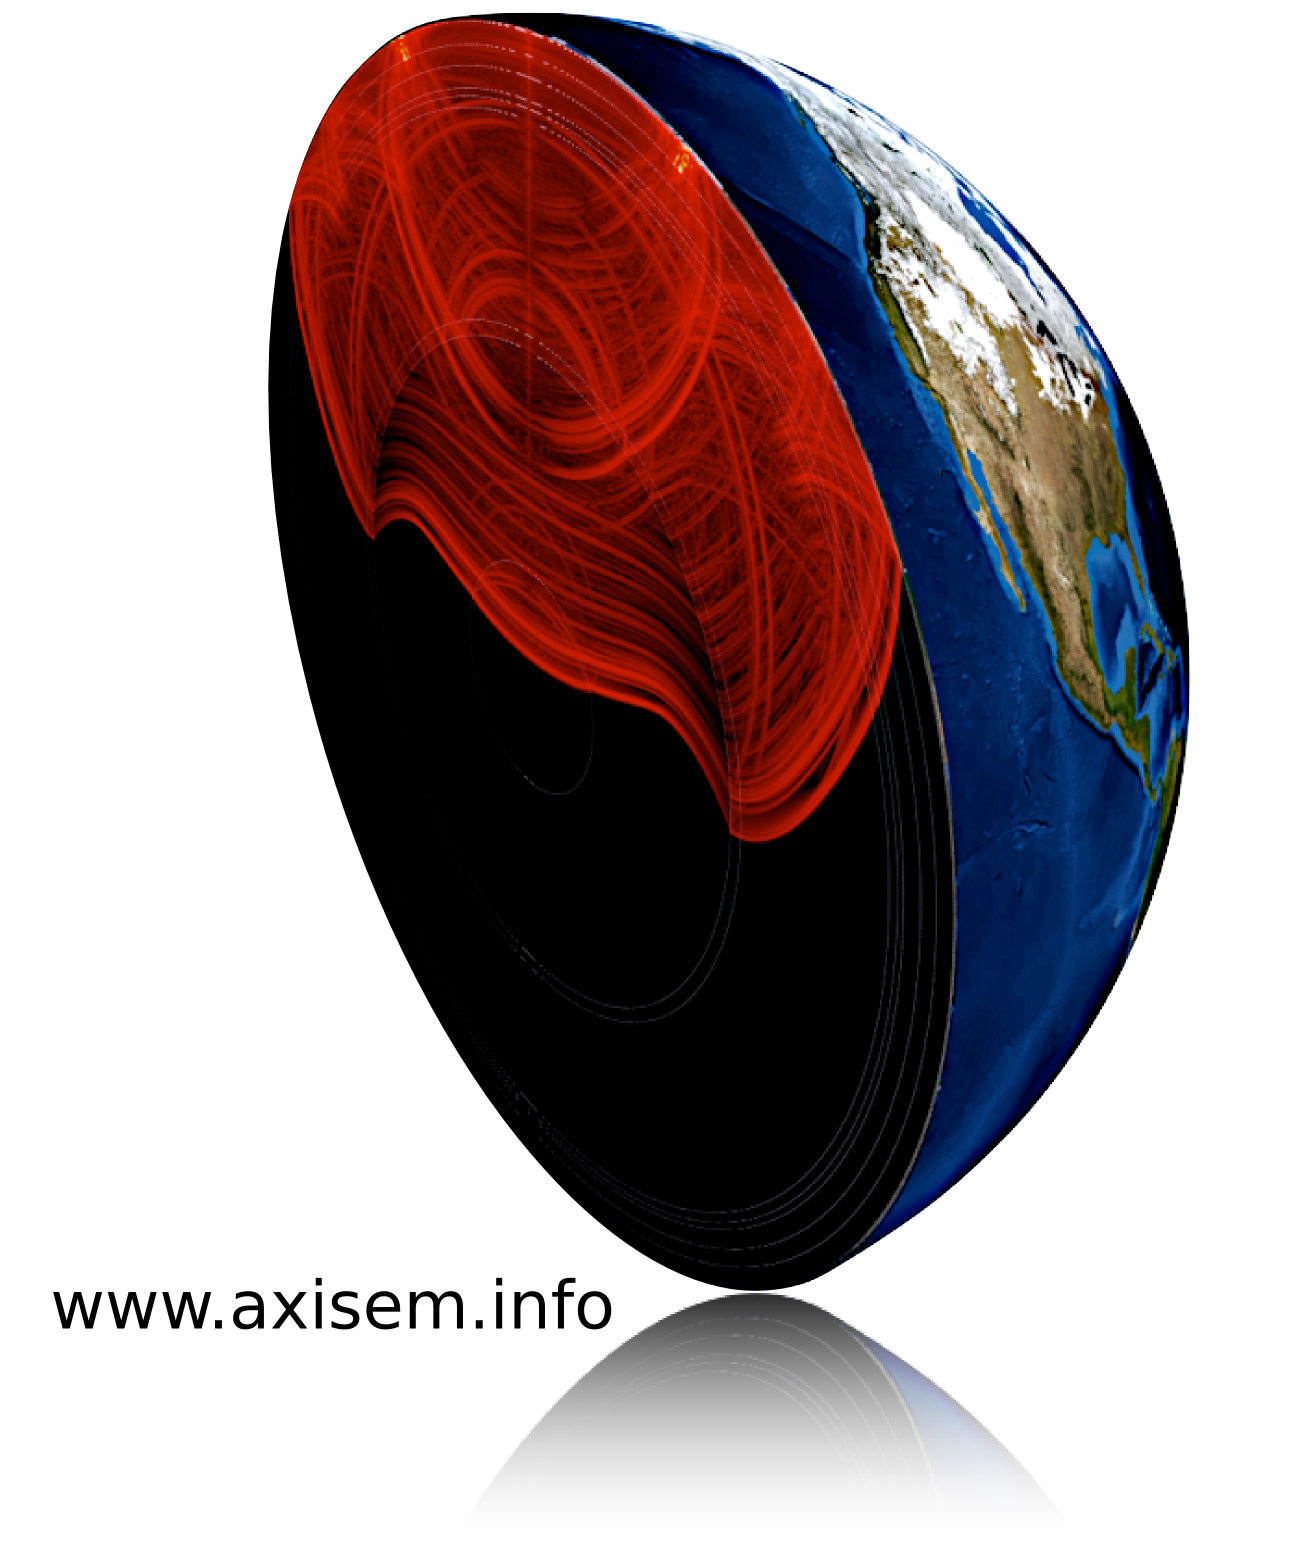
\includegraphics[width=\textwidth]{Axisem2png.png}
            \end{center}
        \end{minipage}
        &
        \begin{minipage}{0.6\textwidth}
            \begin{center}
                \title{}
                \LARGE{ \textbf{\sc AxiSEM Tutorial}}
                \vspace*{0.6cm}\\
                {\large 
                Kasra Hosseini\textsuperscript{1)}, 
                Martin van Driel\textsuperscript{2)},
                Simon St\"{a}hler\textsuperscript{1)}, \\
                \vspace*{-0.3cm}
                Lion Krischer\textsuperscript{1)},
                Tarje Nissen-Meyer\textsuperscript{3)}}
                \vspace*{0.3cm}\\
                {\small \textsuperscript{1)} LMU Munich, \textsuperscript{2)} ETH Zurich, 
                \textsuperscript{3)} Oxford University \\
                {\large Fairbanks, Alaska, July 15th 2013}}
            \end{center}
        \end{minipage}
    \end{tabularx}
\end{center}
   

%
\section{Tutorial Overview}
%
\subsection*{ObsPy \small{(http://www.obspy.org)}}
\vspace{1ex}
\begin{center}
    \begin{tabularx}{\textwidth}{lX}
        \begin{minipage}{0.3\textwidth}
            \begin{center}
                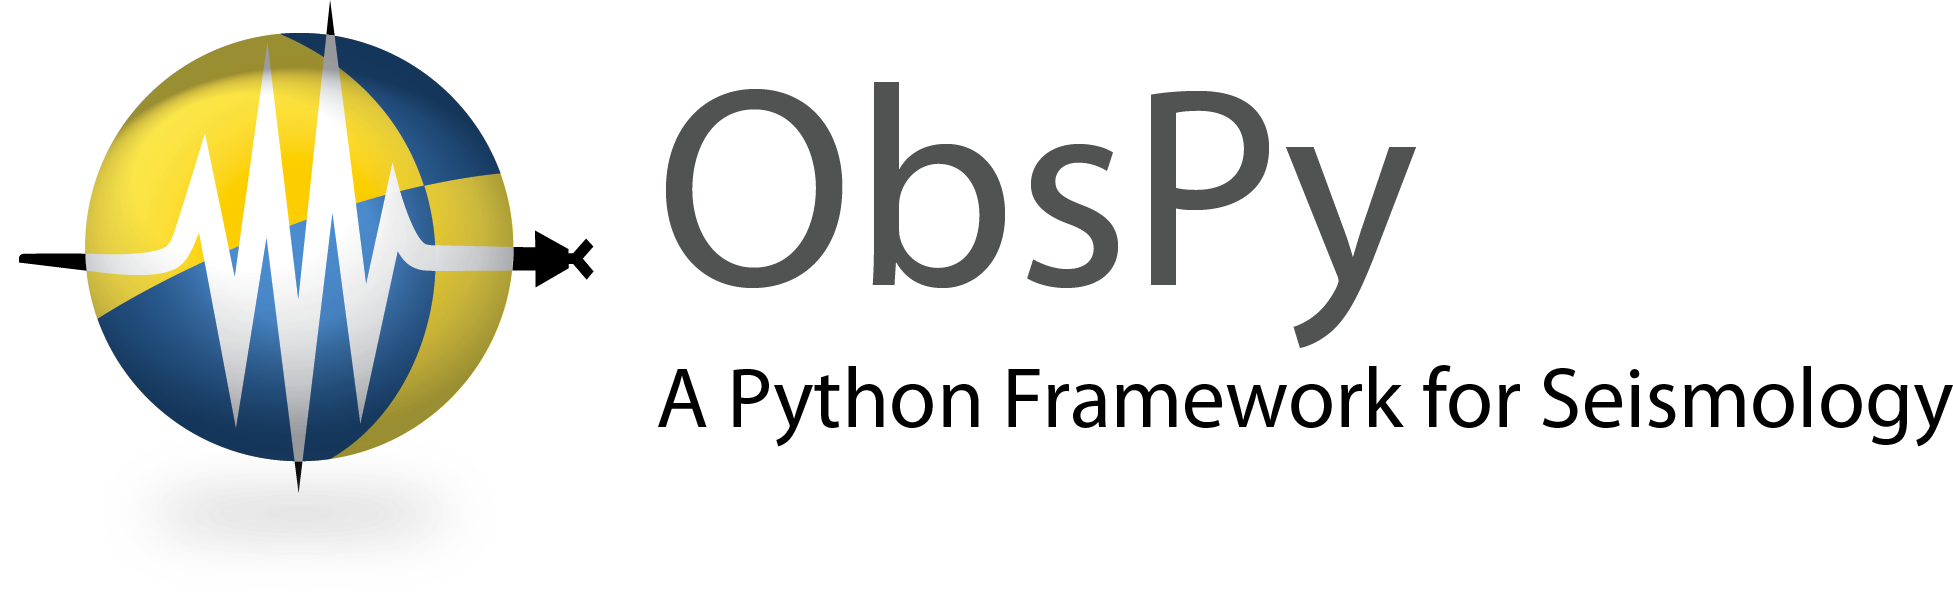
\includegraphics[width=0.9\columnwidth]{obspy.png}
            \end{center}
        \end{minipage}
        &
        \begin{minipage}{0.65\textwidth}
            ObsPy is a community-driven, open-source project dedicated to
            provide a Python framework for processing seismological data. It
            provides parsers for common file formats, clients to access data
            centers and seismological signal processing routines which allow
            the manipulation of seismological time series. The goal of the
            ObsPy project is to facilitate rapid application and workflow
            development for seismology.
        \end{minipage}
    \end{tabularx}
\end{center}


Some of the tools employed in this tutorial use ObsPy but the tutorial
does not have a formal introduction to ObsPy due to temporal
constraints. The VirtualBox image contains an extensive amount of
training material for Python, ObsPy and some third party libraries
intended to get you started. Furthermore one of the core developers of
ObsPy is present and available for questions. You can find all material related
to ObsPy at \ttilde\verb|/Desktop/ObsPy|.
%
\subsection*{AxiSEM - Hands On}
The goal of this initial task is to familiarize users with the basic
principles behind AxiSEM, its input/output structures and
peculiarities such as post-processing. An end-to-end approach (meshing to
wavefield movie and seismograms) will be conducted for long-period
settings within the virtual box.
%
\subsection*{Data and Synthetics: ObsPy, AxiSEM and SPECFEM}
The main goal of this part of the tutorial is to use AxiSEM for realistic
scenarios, compare the results with real seismograms and explore the effects of
source parameters and background models on the waveforms. In particular, we will
learn how to:

\begin{itemize}
    \item Load data with ObsPy and plot seismograms.
    \item compare AxiSEM and SPECFEM synthetics with data including
        different frequency ranges and background model.
    \item analyze the influence of different source mechanisms on waveforms.
\end{itemize}


\subsection*{Virtual Box content}
On the desktop you find four folders:
\begin{itemize}
    \item \verb|ObsPy|: ObsPy training material.
    \item \verb|axisem|: AxiSEM source code and input files ready for the tutorial.
    \item \verb|EVENTS|: Data and precomputed synthetics for three events and various background models.
    \item \verb|VIDEOS|: Illustrative 3D wave propagation video and high-resolution snapshots thereof.
\end{itemize}

\newpage

\section{AxiSEM - Hands On}

\subsection*{The AxiSEM Concept}

\begin{center}
    \begin{minipage}[t]{0.4\paperwidth}
        Source Decomposition:\\
        \begin{minipage}[c]{0.1\paperwidth}
            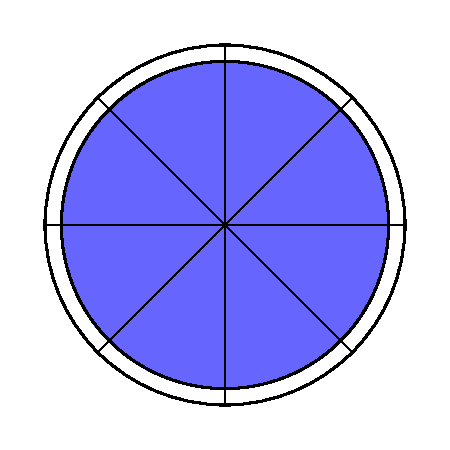
\includegraphics[width=\textwidth]{radpat_mono.pdf}%
        \end{minipage}%
        \begin{minipage}[c]{0.4\paperwidth}
            $\scriptsize{\vec u = \vec u (s,z)}$ \\
        \end{minipage}
    
        \begin{minipage}[c]{0.1\paperwidth}
            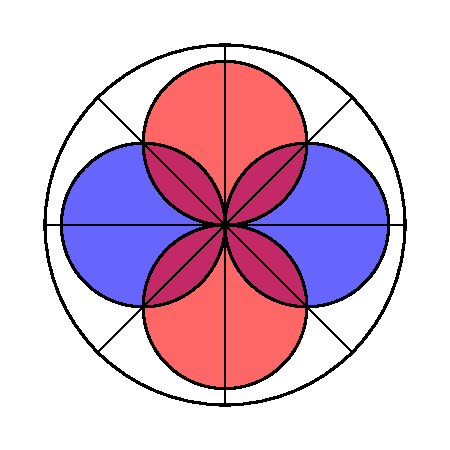
\includegraphics[width=\textwidth]{radpat_di.pdf}
        \end{minipage}%
        \begin{minipage}[c]{0.4\paperwidth}
            $\scriptsize{\vec u = \vec u (s,z)} \cdot f(\sin\phi, \cos\phi)$ \\
        \end{minipage}
    
        \begin{minipage}[c]{0.1\paperwidth}
            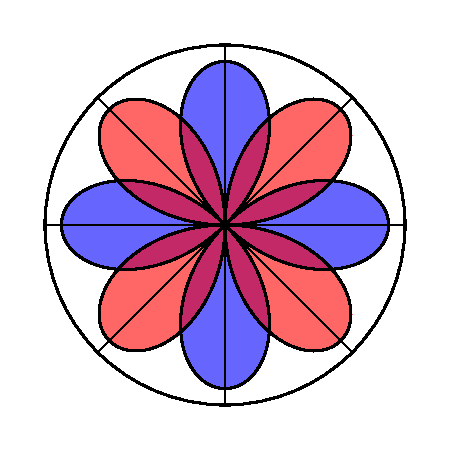
\includegraphics[width=\textwidth]{radpat_quad.pdf}
        \end{minipage}%
        \begin{minipage}[c]{0.4\paperwidth}
            $\scriptsize{\vec u = \vec u (s,z)} \cdot f(\sin(2\phi), \cos(2\phi))$ \\
        \end{minipage}%
    \end{minipage}%
    \begin{minipage}[t]{0.25\paperwidth}
        2D numerical problems:
    
        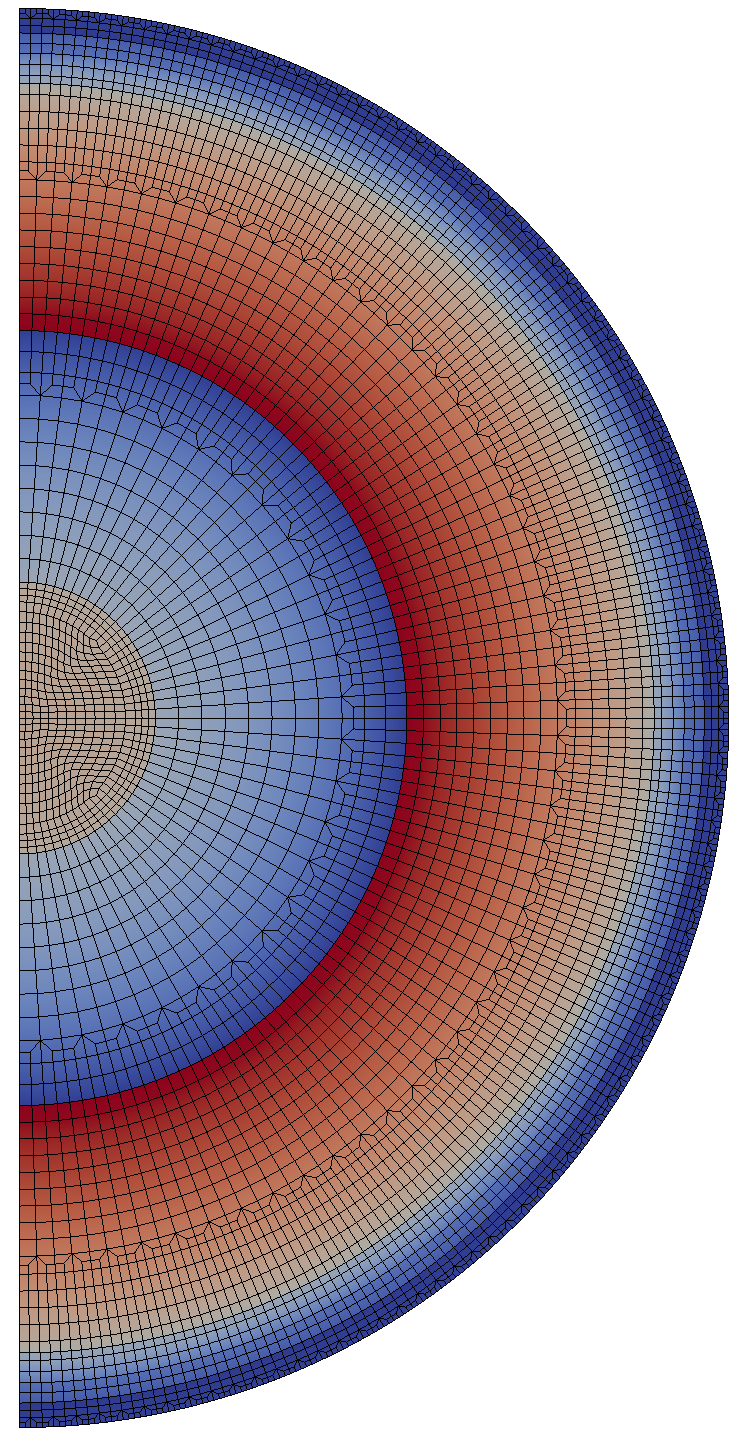
\includegraphics[width=.7\textwidth]{mesh.png}
    \end{minipage}%
\end{center}

The basic idea behind AxiSEM is to take advantage of axial symmetry with respect
to an axis going through the center of the earth and the source. In such axisymmetric 
models, the response to a moment tensor or single force point source can be expanded in a
series of multipoles (mono-, di- and quadrupole). The dependence of the wavefield on
azimuth $\phi$ can be solved analytically and the remaining 2D problems (four of them for
a full moment tensor source) are solved numerically using a spectral element approach.


\subsection*{MESHER - generate a Mesh}

\begin{enumerate}
    \item Open a terminal, go to the \ttilde\verb|/Desktop/axisem/MESHER| folder and open
    the \verb|inparam_mesh| file with your favourite editor:
    %
    \begin{verbatim}
    $ cd Desktop/axisem/MESHER
    $ vi inparam_mesh
    \end{verbatim}
    %
    The parameters should be readily set, but you might want to double check and verify:
    %
    \begin{verbatim}
    BACKGROUND_MODEL    'prem_ani_light'
    DOMINANT_PERIOD     100.0
    NCPU                1
    WRITE_VTK           true
    COARSENING_LAYERS   2
    \end{verbatim}
    %
    The file should be self-explanatory. NB: Models without crust ('light') allow for a
    larger time step and hence run a lot faster on the box. The virtual box only has a
    single processor, so parallelization does not speed up the simulation.

    \item Run the mesher, and watch the progress:
    %
    \begin{verbatim}
    $ ./submit.csh
    $ tailf OUTPUT
    \end{verbatim}
    %
    The meshing should be really fast for the chosen parameters. Wait for 
    \verb|....DONE WITH MESHER !| to appear.

    \item Take a look at the mesh with paraview
    \begin{verbatim}
    $ paraview
    \end{verbatim}
    %
    Open one of the vtk files in the subfolder \verb|Diags|, e.g.\
    \verb|mesh_vp.vtk| and click apply in the properties panel on the left (you
    might get an OpenGL Error on the virtual box, which you can ignore). To see
    the mesh, change the representation from 'surface' to 'surface with edges'
    (On some host systems, the dropdown menu seems to be messed up, in that
    case go to the 'Display' context in the 'Properties' panel on the left. If
    the plot appears all yellow, click on play).  You can open other vtk files
    to look at other properties of the model and the mesh. You might need to
    rescale the color range by clicking on the left-right arrow symbol in the
    top left.

    \begin{center}
    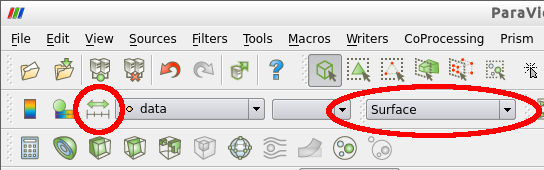
\includegraphics[height=30mm]{paraview.png}
    \hspace{5mm}
    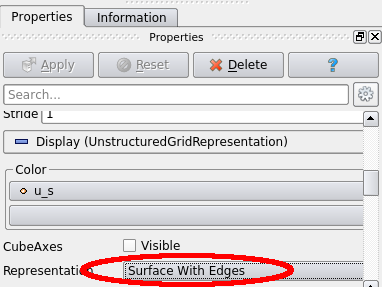
\includegraphics[height=30mm]{paraview3.png}
    \end{center}
        
    \item Move the mesh to the solver directory and give it a meaningful name:
    \begin{verbatim}
    $ ./movemesh.csh prem_ani_light_100s
    \end{verbatim}

\end{enumerate}

\subsection*{SOLVER - solve the elastic wave equation}
    
\begin{enumerate}
    \item Go to the \ttilde\verb|/Desktop/axisem/SOLVER| folder and open the
    \verb|inparam_basic| file with your favourite editor:
    %
    \begin{verbatim}
    $ cd ../SOLVER
    $ vi inparam_basic
    \end{verbatim}
    %
    The parameters should be readily set, but you might want to double check and verify:
    %
    \begin{verbatim}
    SIMULATION_TYPE     single
    SEISMOGRAM_LENGTH   1800.
    RECFILE_TYPE        stations 
    MESHNAME            prem_ani_light_100s
    ATTENUATION         true 
    SAVE_SNAPSHOTS      true  
    \end{verbatim}
    %
    \item First, we are taking a look at a basic sourcetype: a vertical dipole, which has
    a monopole radiation pattern. This is set by \verb|SIMULATION_TYPE single| and defined
    in the \verb|sourceparams.dat| file. Run the solver, giving the run a meaningful name:
    %
    \begin{verbatim}
    $ ./submit.csh prem_ani_light_100s_mzz
    \end{verbatim}
    %
    This command compiles the code if needed and starts the simulation. You can observe
    the progress in the outputfile:
    %
    \begin{verbatim}
    $ cd prem_ani_light_100s_mzz
    $ tailf OUTPUT_prem_ani_light_100s_mzz
    \end{verbatim}
    %
    Once the run is finished, take a look at the wavefield with \verb|paraview|: open
    the \verb|prem_ani_light_100s_mzz/| \verb|Data/xdmf_xml_0000.xdmf|
    file and click apply. Go to the last snapshot and rescale the color range,
    then click on play to see the wave propagate.  You can also choose
    different components of the wavefield or the absolute value.  For paraview
    experienced users: choose absolute value and a logarithmic colorscale to
    see all wave types at once (e.g.\ 'black body radiation' looks nice).  You
    can find a 5s period movie of these snapshots in the \verb|VIDEOS| folder on
    the desktop (use \verb|gpicview| to open the \verb|.png| files and
    \verb|gnome-mplayer| to open the movie \verb|SeismicWavePropagation.mov|).
   
    \begin{center}
    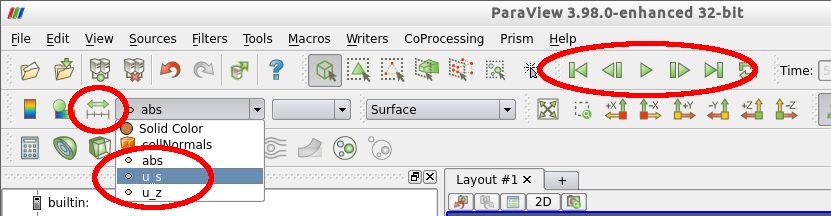
\includegraphics[width=110mm]{paraview2.png} \hspace{5mm}
    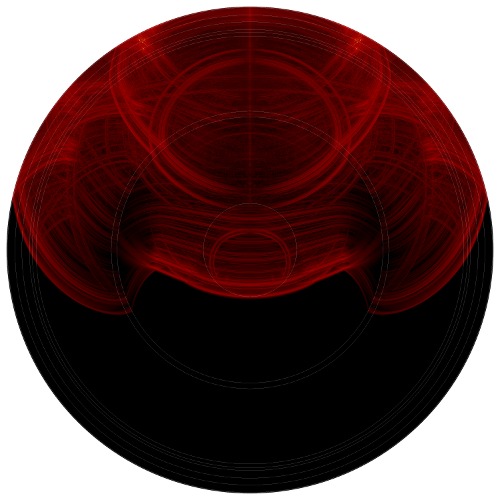
\includegraphics[width=40mm]{0600.png}
    \end{center}

    \item Now simulate seismograms for a full moment tensor source: the source is defined
    in the \verb|CMTSOLUTION| file and the one referred to as 'event-1' in the later tasks.
    Stations are defined in the \verb|STATIONS| file. Go back to the \verb|SOLVER|
    directory and change the \verb|inparam_basic| file such that:
    %
    \begin{verbatim}
    SIMULATION_TYPE     moment
    SAVE_SNAPSHOTS      false
    \end{verbatim}
    %
    Run the solver, giving the run a meaningful name:
    %
    \begin{verbatim}
    $ ./submit.csh prem_ani_light_100s_event1
    \end{verbatim}
    %
    This command compiles the code if needed and starts four simulations at once, each
    simulating a basic source type (two monopoles, a dipole and a quadrupole, for details
    see Nissen-Meyer et al 2007). You can observe the progress in the outputfiles in
    each job's subdirectory
    %
    \begin{verbatim}
    $ cd prem_ani_light_100s_event1
    $ tailf MZZ/OUTPUT_MZZ
    \end{verbatim}
    %
    Once all the jobs are done (check with \verb|htop|), you can proceed with
    postprocessing.
    
\end{enumerate}
    

\subsection*{POSTPROCESSING - rotate and sum seismograms and wavefields}

Postprocessing is a key feature of AxiSEM: the source mechanism and source time function
can be modified without redoing the more expensive simulation.

\begin{enumerate}
    \item For the previous simulation, the contribution of the elemental sources needs
    to be summed up to get seismograms for a full moment tensor source. In the
    main rundirectory (\verb|prem_ani_light_100s_event1|) open the file
    \verb|param_postprocessing|. It should contain these settings (auto generated by the
    solver):
    %
    \begin{verbatim}
    REC_COMP_SYS    enz
    CONV_PERIOD     100.0000
    CONV_STF        gauss_0
    \end{verbatim}
    %
    The source mechanism (depth and location cannot be changed in postprocessing) is read
    from the \verb|CMTSOLUTION| file in the same directory. Start the postprocessing:
    %
    \begin{verbatim}
    $ ./postprocessing.csh
    \end{verbatim}
    %
    The resulting seismograms and plots can be found in the directory 
    \verb|Data_Postprocessing|. Seismograms can be viewed with
    %
    \begin{verbatim}
    $ cd Data_Postprocessing/GRAPHICS
    $ gpicview <filename.gif>
    \end{verbatim}
    %
    For a nice overview, you can use \verb|google-earth| (might not run on all computers
    and depends on internet connection). Open the \verb|googleearth_src_rec_seis.kml| file
    in the \verb|Data_Postprocessing/| directory (double check the exact path,
    google-earth might have something older from history which is quite confusing).
    You should now see the earthquake and the receivers in the places menu on the left.
    
    \begin{center}
    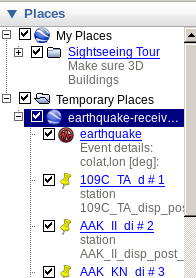
\includegraphics[height=70mm]{google-earth.png}
    \hspace{5mm}
    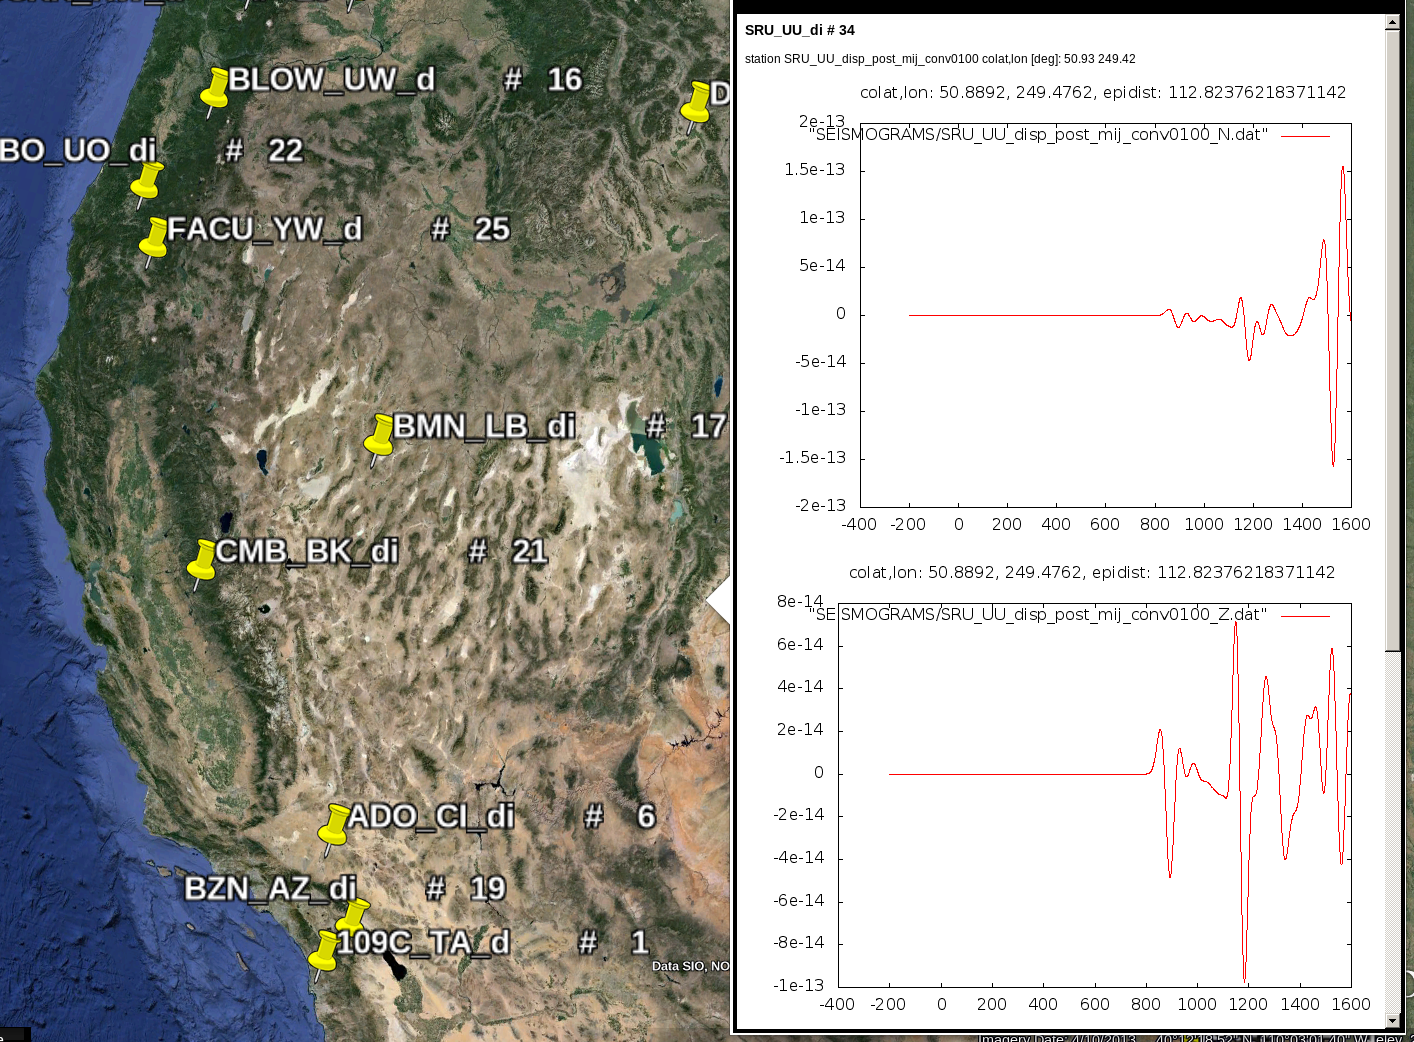
\includegraphics[height=70mm]{google-earth2.png}
    \end{center}

    Click on the stations or source to see more...

\end{enumerate}


%\emph{Low-frequency simulation at period 50/100 s (20min)}
%\begin{enumerate}
%    \item change AxiSEM input parameters to run this scenario, submit job
%    \item check mesh, background model, source-receiver geometry (google earth)
%    \item post processing on 50s run: filter, sum, rotate, movie snapshots
%\end{enumerate}

\newpage

\section{Data and Synthetics: ObsPy, AxiSEM and SPECFEM}
The main goal of this part of the tutorial is to use AxiSEM for realistic scenarios, 
compare the results with real seismograms and 3D synthetics and 
explore the effects of source parameters and background models on the waveforms. 
% In case that you want more information, 
% refer to Appendix-5 in which a complete example with all the commands and results is presented.
For a brief walk-through, follow this: \\

Start from within the \ttilde\verb|/Desktop/EVENTS/| directory:

\begin{enumerate}
    
    \item Plot one of the events (listed in EVENTS directory, we choose EVENT-1
    in this example):
    
    \begin{verbatim}
    $ plot_station_event_distribution.py EVENT-1
    \end{verbatim}
    * For more information on the folder structure of your VirtualBox image,
    refer to Appendix-2.
    
    \item To get an overview of both real data and AxiSEM synthetics 
    (e.g.\ \textit{PREM\_ANISO} for 5 seconds dominant period) [Figure-1]:
    \begin{verbatim}
    $ plot_seismograms.py EVENT-1/AXISEM/PREM_ANISO_5sec
    \end{verbatim}
    
    \item Window the waveforms arounf Pdiff and PKiKP seismic phases and plot
    the seismograms (compared with real data):
    \begin{verbatim}
    $ plot_seismograms.py EVENT-1/AXISEM/PREM_ANISO_5sec Pdiff
    $ plot_seismograms.py EVENT-1/AXISEM/PREM_ANISO_5sec PKiKP
    \end{verbatim}
    
    \item Change the filter in the
    \ttilde\verb|/Desktop/EVENTS/SCRIPTS/plot_seismograms.py| script and
    compare the results with SPECFEM3D [Figure-2]:
    
    Note: for changing the filter, open \textit{plot\_seismograms.py} and
    change values at top of the file. \\
    Note: resolution in SPECFEM3D seismograms is 17 - 500 sec.
    \begin{verbatim}
    $ plot_seismograms.py EVENT-1/AXISEM/PREM_ANISO_5sec Pdiff specfem3d
    $ plot_seismograms.py EVENT-1/AXISEM/PREM_ANISO_5sec PKiKP specfem3d
    \end{verbatim}
    
    \item Compare the results for two different background models
    (\textit{PREM\_ANISO\_5sec} with \textit{IASP91\_5sec)} e.g.\ Pdiff phase:
    
    \begin{verbatim}
    $ plot_seismograms.py EVENT-1/AXISEM/PREM_ANISO_5sec Pdiff EVENT-1/AXISEM/IASP91_5sec
    \end{verbatim}
    
    \item Change the filter, as explained in step 4, and repeat step 5.
    
    \item Compare the seismograms calculated for two different source
    mechanisms (\textit{PREM\_ANISO\_5sec} and \\
    \textit{PREM\_ANSIO\_5sec\_GCMT}) for Pdiff phase [Figure-3]:
    
    Note: for more information about the source parameters, refer to Appendix-1.\\
    Note: depth and location of the source can not be changed.
    \begin{verbatim}
    $ plot_seismograms.py EVENT-1/AXISEM/PREM_ANISO_5sec Pdiff 
    EVENT-1/AXISEM/PREM_ANISO_5sec_GCMT
    \end{verbatim}
    
    \item Try different filter settings and compare the results.
    (Note: dominant period in synthetic seismograms is 5 sec.)
    
    \item Find the time shift between the synthetics and real data (maximum of
    cross-correlation function), shift the synthetics accordingly and plot the results:
    
    \begin{verbatim}
    $ plot_seismograms.py EVENT-1/AXISEM/PREM_ANISO_5sec Pdiff shift_synthetics
    \end{verbatim}
    
    \item Map the calculated time shifts in step 9 on the station locations:
    
    \begin{verbatim}
    $ plot_travel_time_map.py EVENT-1
    \end{verbatim}

\end{enumerate}

\newpage
\begin{figure}[H]
    \centering
    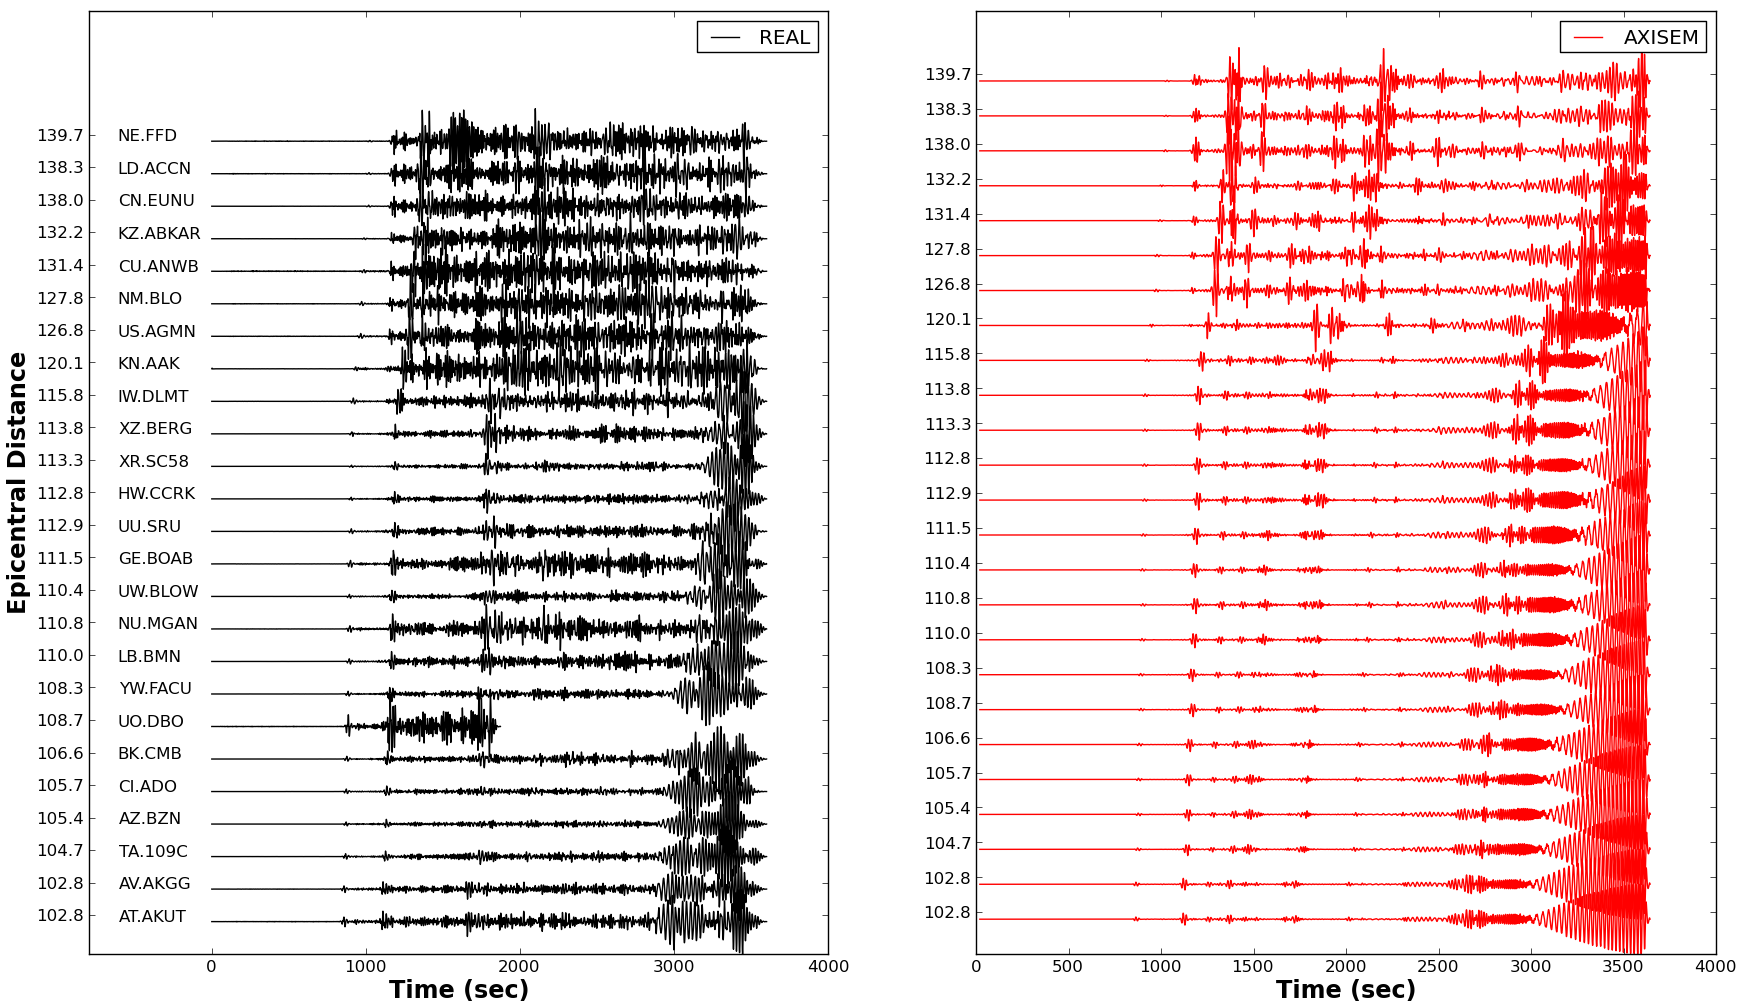
\includegraphics[width=1.\linewidth]{AXISEMTutorial-fig007.png}
    \begin{center}
    {\small{}Figure 1: Real and AXISEM waveforms for EVENT-1.}
    \end{center}
\end{figure}


\begin{figure}[H]
    \centering
    \begin{minipage}{.5\textwidth}
        \centering
        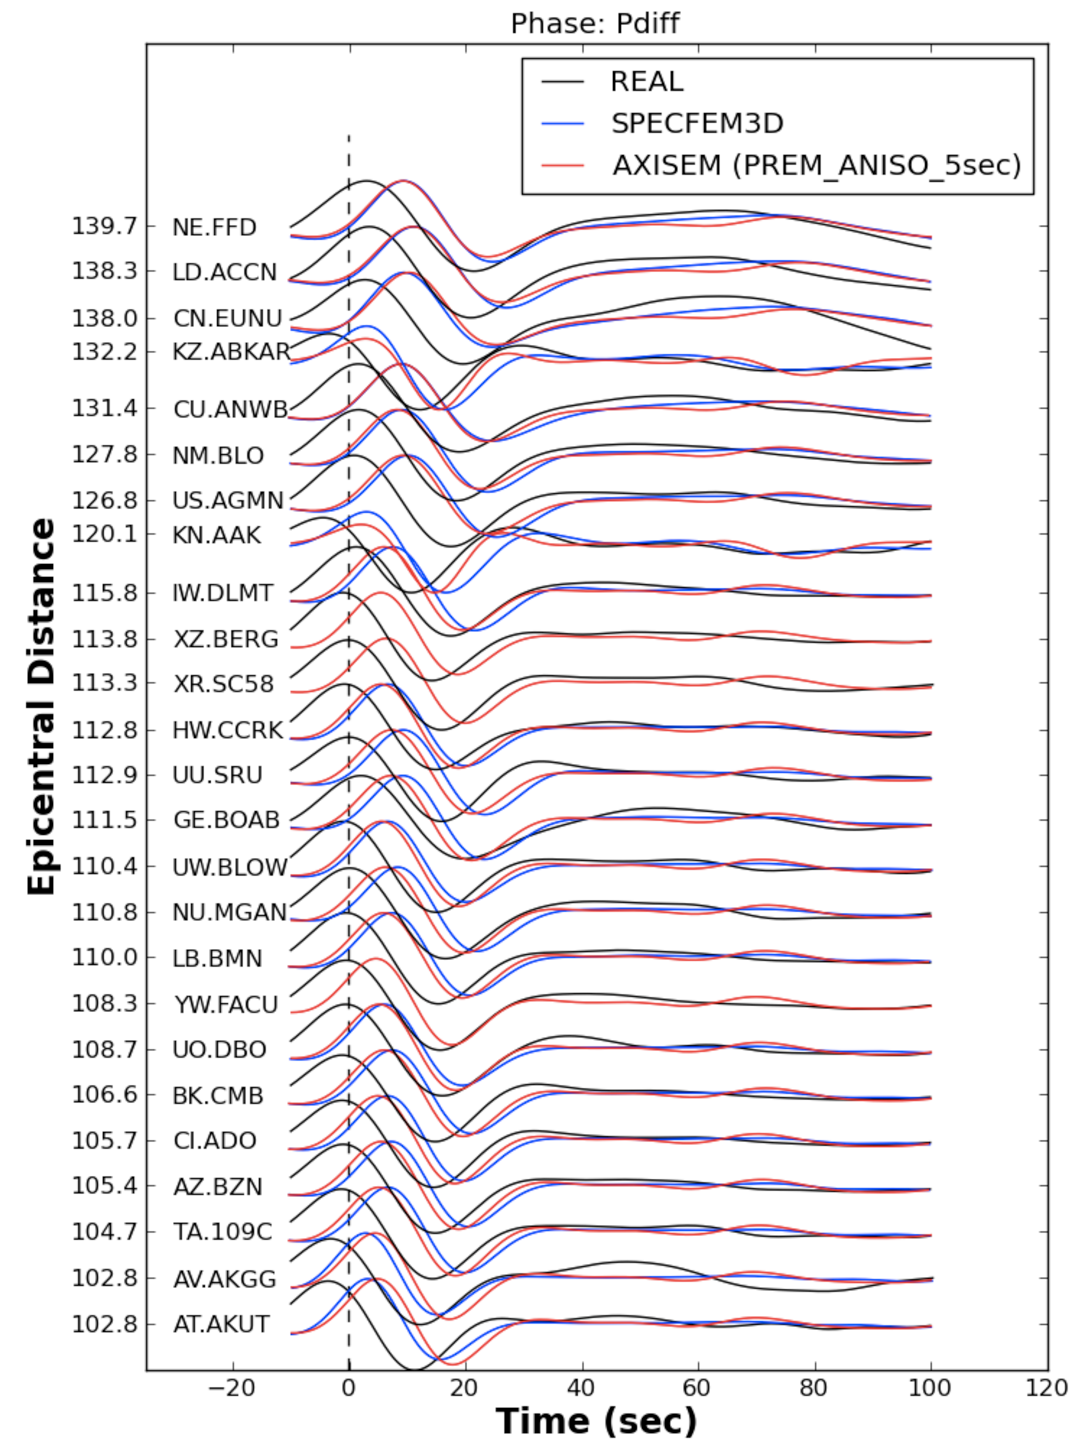
\includegraphics[width=0.9\linewidth]{AXISEMTutorial-fig010.pdf}
        {\small{}Figure 2: Comparison between real, AXISEM and SPECFEM3D waveforms for 
        Pdiff phase. \\ Filter: 20 - 100 sec.}
    \end{minipage}%
    \begin{minipage}{.5\textwidth}
        \centering
        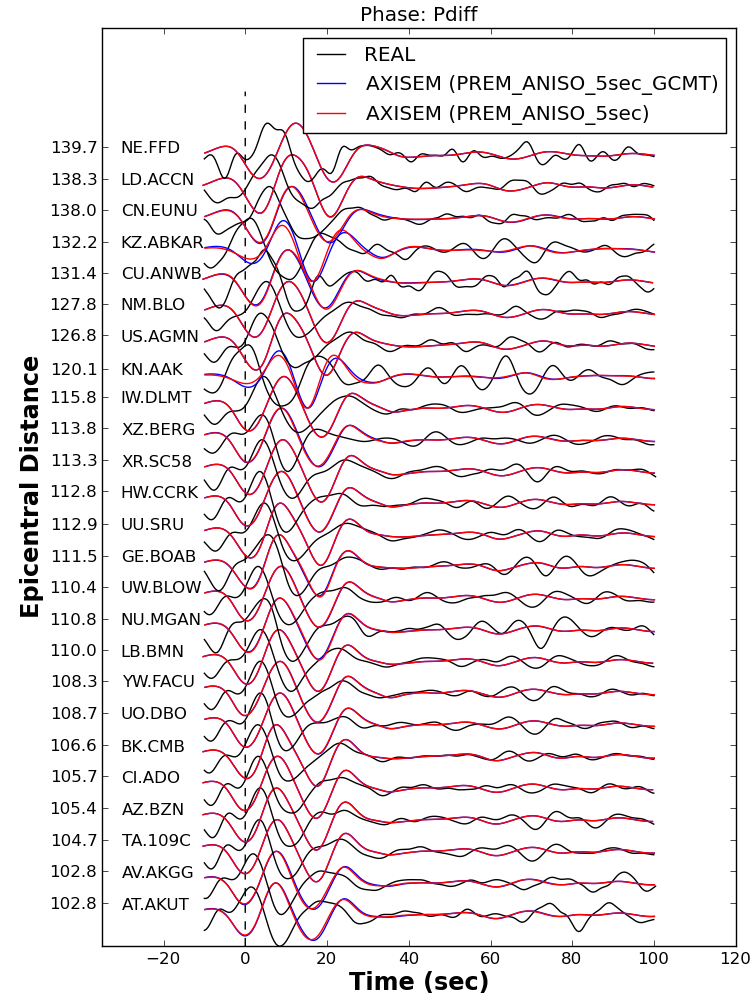
\includegraphics[width=0.9\linewidth]{AXISEMTutorial-fig014.png}
        {\small{}Figure 3: Comparison between real and AXISEM waveforms for two different 
        source parameters (Pdiff). \\ Filter: 5 - 20 sec.}
    \end{minipage}
\end{figure}


\newpage
\appendix
\section{APPENDIX-1: Events}

Three events are selected for this tutorial (Figure-A1) with the following source 
characteristics:

\begin{center}
%%\begin{figure}[htbp]
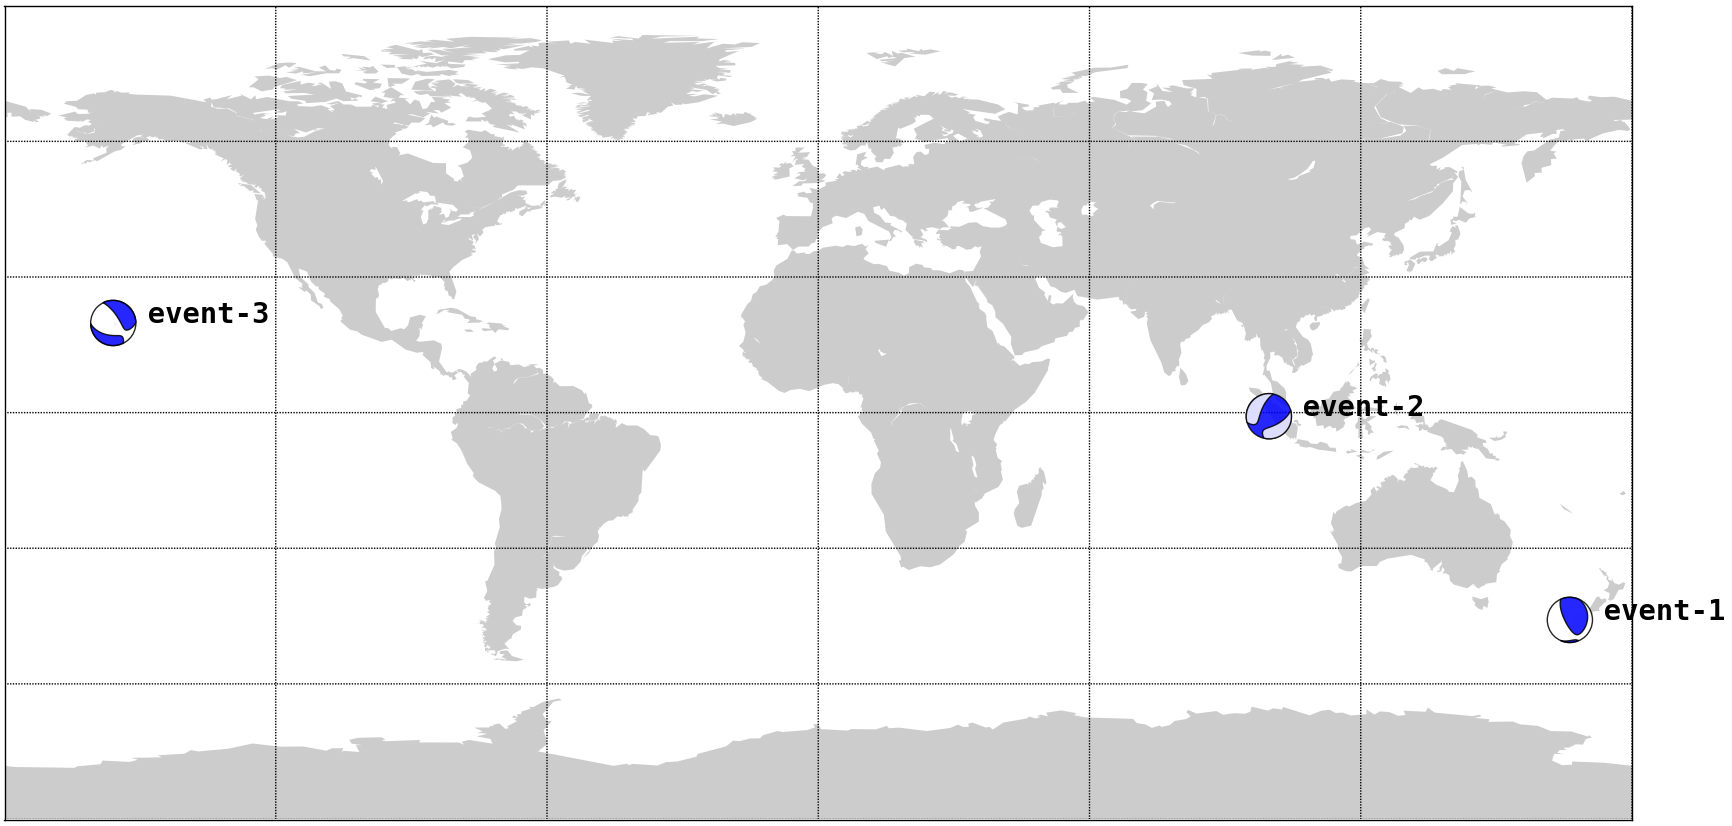
\includegraphics[width=372pt, height=178pt, keepaspectratio=true]{AXISEMTutorial-fig001.png}
%%\caption{This should be the caption for \texttt{AXISEMTutorial-fig001.png}.}
%%\end{figure}

{\small{}Figure A1: beach ball diagrams of event-1 to event-3 (based on GCMT catalog)}

\vspace{1cm}
%%\begin{figure}[htbp]
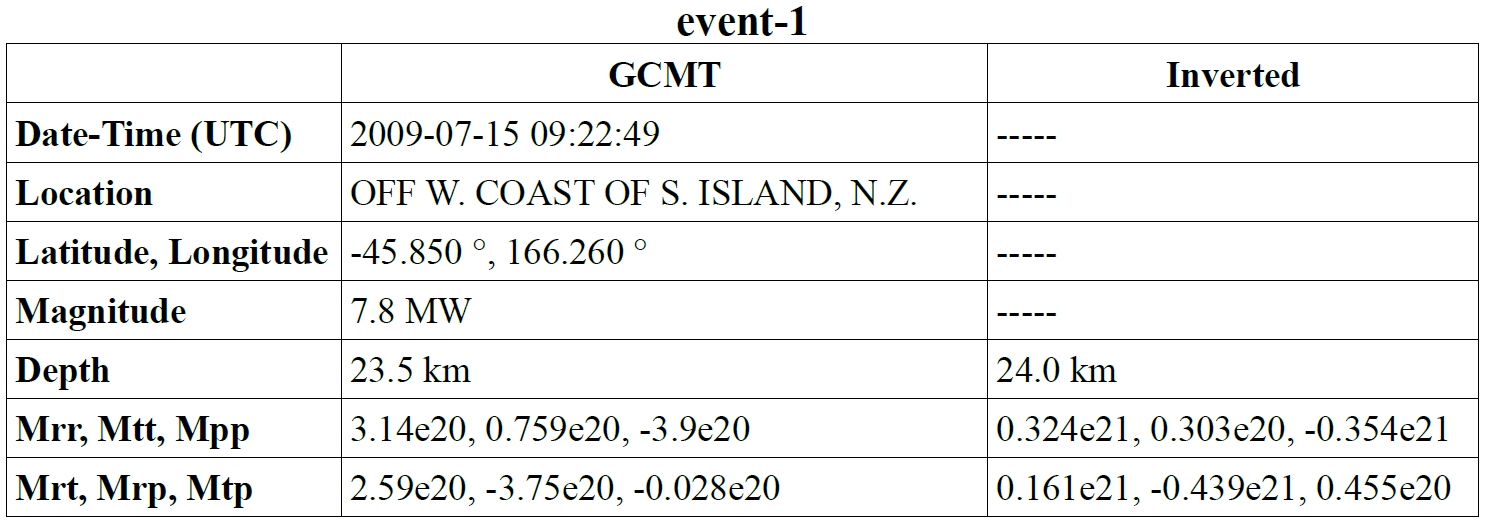
\includegraphics[width=312pt, height=110pt, keepaspectratio=true]{AXISEMTutorial-fig002.png}
%%\caption{This should be the caption for \texttt{AXISEMTutorial-fig002.png}.}
%%\end{figure}

\vspace{1cm}
%%\begin{figure}[htbp]
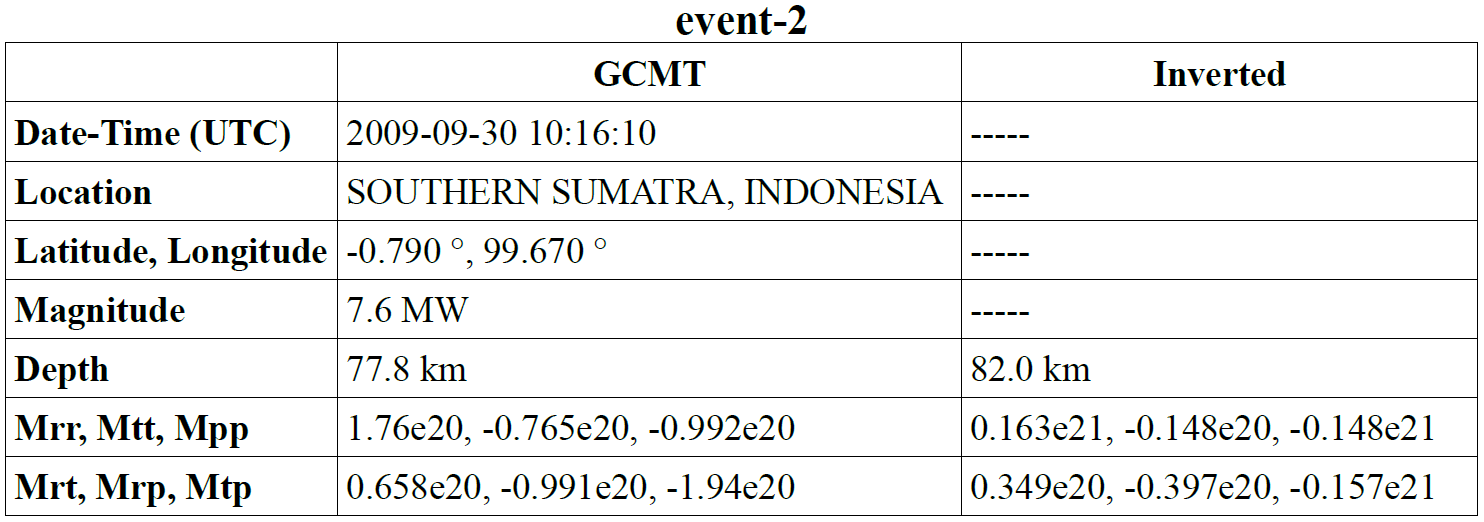
\includegraphics[width=312pt, height=110pt, keepaspectratio=true]{AXISEMTutorial-fig003.png}
%%\caption{This should be the caption for \texttt{AXISEMTutorial-fig003.png}.}
%%\end{figure}

\vspace{1cm}
%%\begin{figure}[htbp]
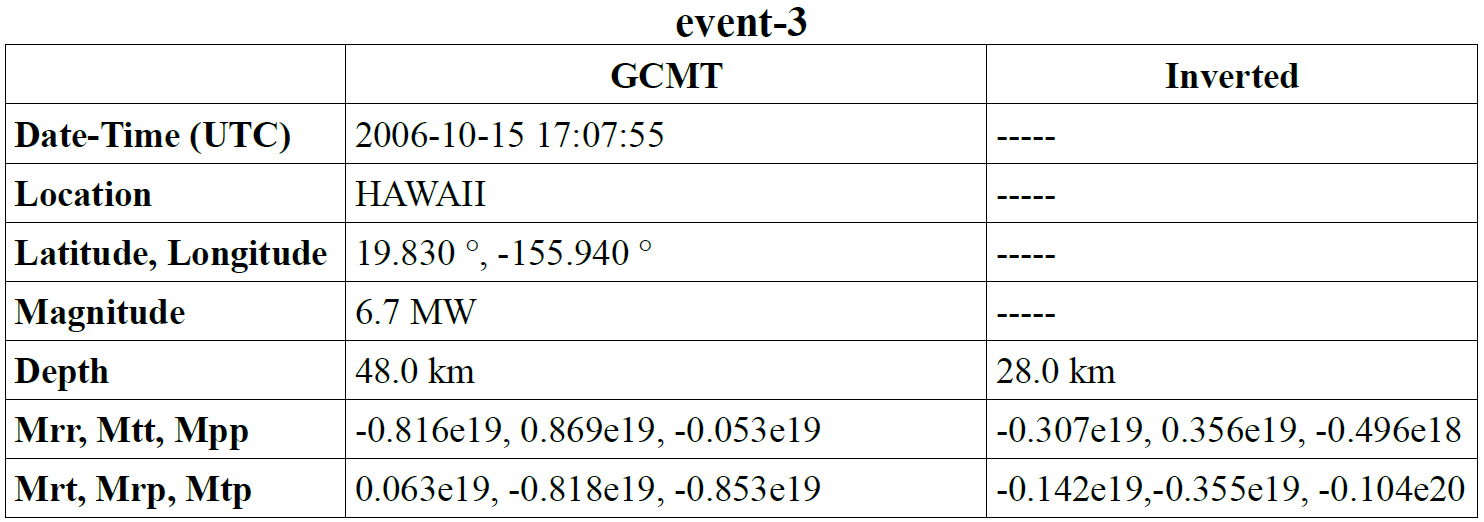
\includegraphics[width=312pt, height=110pt, keepaspectratio=true]{AXISEMTutorial-fig004.png}
%%\caption{This should be the caption for \texttt{AXISEMTutorial-fig004.png}.}
%%\end{figure}

\end{center}


%\baselineskip=13pt
%\leftskip=0pt

\newpage

\section{APPENDIX-2: Folder structure}

Figure A2 shows how the events (and their meta-data), waveforms and scripts are 
organized in the Virtual-box:

\begin{center}
%%\begin{figure}[htbp]
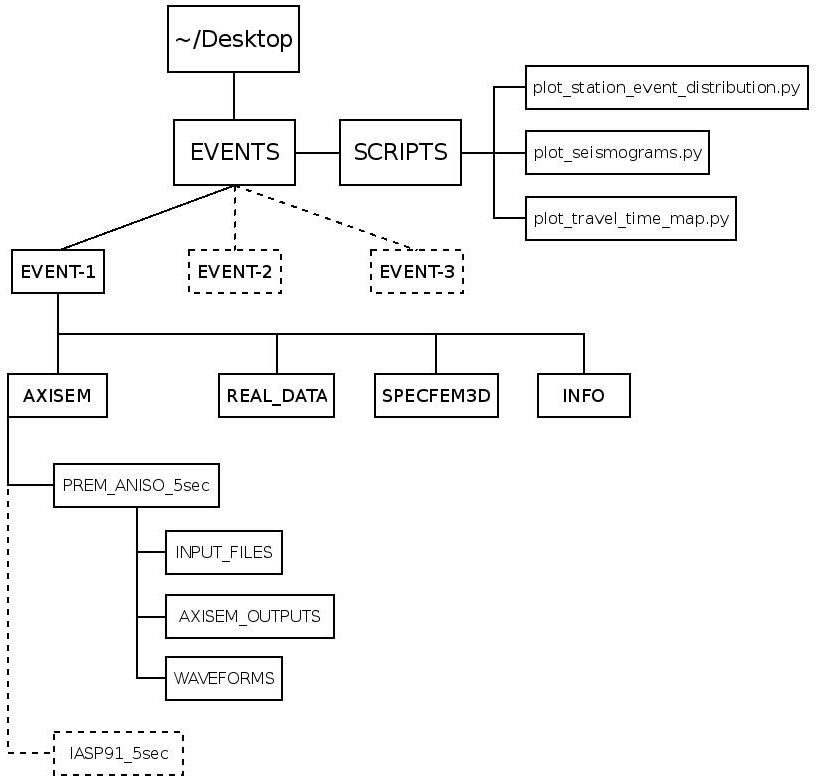
\includegraphics[width=334pt, height=362pt, keepaspectratio=true]{Folder_structure.jpeg}

Figure A2: Folder structure
%%\end{figure}
\end{center}

In \textit{SCRIPTS} directory, there are three python scripts that we use here:

\begin{enumerate}
    \item \textbf{plot\_station\_event\_distribution.py}: maps event and stations of an
    event directory.
    \item \textbf{plot\_seismograms.py}: plotting/filtering seismograms for comparison purposes.
    \item \textbf{plot\_travel\_time\_map.py}: project the time shift measured by cross
    correlating the AXISEM waveforms and real data.
\end{enumerate}

In \textit{EVENTS} directory, there are three events, each with the following
sub-directories:

\begin{enumerate}
    \item \textbf{AXISEM}: contains seismograms simulated by AXISEM with
    the required PyAxi (Appendix-3) input files (INPUT\_FILES) to re-produce them.
    \item \textbf{REAL\_DATA}: seismograms retrieved from \textit{IRIS. }(refer to
    APPENDIX-4)
    \item \textbf{SPECFEM3D}: waveforms simulated by \textit{SPECFEM3D} for comparison purposes. (downloaded from\textit{ IRIS}, refer to APPENDIX-4)
    \item \textbf{INFO}: information about the event and stations: \textit{event\_1.xml} and
    \textit{STATIONS}.
\end{enumerate}


\newpage
\section{APPENDIX-3: A Quick Guide to PyAxi}

PyAxi is a Python script developed as an interface for AXISEM. All the options 
available in AXISEM are included in only one input file (\textit{inpython.cfg}). By running 
the script, all the necessary steps (MESHER, SOLVER and Post-Processing) will be 
done automatically. \\

All you should do to run PyAxi for an input file (\textit{inpython.cfg}) and station list 
(STATIONS) is:
\begin{verbatim}
    $ python PyAxi <inpython.cfg> <STATIONS>
\end{verbatim}

and the rest should be done automatically. \\
\textit{inpython.cfg} is a conguration file that 
contains all the AXISEM options. To change the input file, open \textit{inpython.cfg} with 
an editor. However, you could find some already prepared \textit{inpython.cfg} files for 
the events in the Virtual-box. (refer to APPENDIX-2 for more information; \textit{INPUT\_FILES} in Figure A2) 
Therefore, to run AXISEM for the provided events (EVENT-1 
and IASP91-5sec as an example), it is enough to replace:

\begin{verbatim}
    <inpython.cfg>: 
    ~/Desktop/EVENTS/EVENT-1/AXISEM/IASP91_5sec/INPUT_FILES/inpython.cfg
    
    <STATIONS>:
    ~/Desktop/EVENTS/EVENT-1/AXISEM/IASP91_5sec/INPUT_FILES/STATIONS
\end{verbatim}

WARNING: this will take ages on the Virtual-box because of the dominant period (5sec) and available computing resources.

\newpage
\section{APPENDIX-4: Retrieving real data and SPECFEM3D seismograms automatically}

{\color{color18} \emph{obspyDMT}} (ObsPy Data Management Tool) is a command line 
tool for retrieving, processing and management of massive seismological data in 
a fully automatic way which could be run in serial or in parallel. \\

This tool is developed to mainly address the following tasks automatically:

1. Retrieval of waveforms (MSEED or SAC), response files and metadata from {\color{color18} \emph{IRIS}} 
and {\color{color18} \emph{ORFEUS}} (via {\color{color18} \emph{ArcLink}}) archives. 
This could be done in \textit{serial} or in \textit{parallel} for single or large 
requests.

2. Supports event-based and continuous requests.

3. Extracting the information of all the events via user-defined options (time 
span, magnitude, depth and event location) from {\color{color18} \emph{IRIS}} and 
{\color{color18} \emph{EMSC}} (European Mediterranean Seismological Centre).

4. Updating the existing archives (waveforms, response files and metadata).

5. Processing the data in \textit{serial} or in \textit{parallel} (e.g. \textit{Tapering, 
removing the trend of the time series, filtering and Instrument correction}).

6. Management of large seismic datasets.

7. Plotting tools (events and/or station locations, Ray coverage (event-station 
pair), epicentral-distance plots for all archived waveforms and seismicity maps).

\vspace{13pt}
Here, we use obspyDMT to retrieve both real data and SPECFEM3D seismograms. For 
more information about this tool please refer to the following webpage:

{\color{color18} \emph{https://github.com/kasra-hosseini/obspyDMT}}  \\

obspyDMT is installed on your virtual machine. By running the following commands, 
the real data used in this tutorial can be retrieved automatically:

\textbf{Event-1:}

\begin{verbatim}
    ./obspyDMT.py --datapath EVENT-1_real --min_date 2009-07-15 --max_date 2009-07-16 
    --min_mag 7.0 --min_depth 20 --list_stas ~/Desktop/EVENT-1/INFO/STATIONS 
    --offset 3600 --req_parallel --arc N
\end{verbatim}

\textbf{Event-2:}

\begin{verbatim}
    ./obspyDMT.py --datapath EVENT-2_real --min_date 2009-09-30 --max_date 2009-10-01 
    --min_mag 7.0 --min_depth 70 --list_stas ~/Desktop/EVENT-1/INFO/STATIONS 
    --offset 3600 --req_parallel --arc N
\end{verbatim}

\textbf{Event-3:}

\begin{verbatim}
    ./obspyDMT.py --datapath EVENT-3_real --min_date 2006-10-15 --max_date 2006-10-16 
    --min_mag 6.0 --min_depth 20 --list_stas ~/Desktop/EVENT-1/INFO/STATIONS 
    --offset 3600 --req_parallel --arc N
\end{verbatim}

Moreover, the SPECFEM3D seismograms can be also retrieved in the same manner:

\textbf{Event-1:}

\begin{verbatim}
    ./obspyDMT.py --datapath EVENT-1 --min_date 2009-07-15 --max_date 2009-07-16 
    --min_mag 7.0 --min_depth 20 --list_stas ~/Desktop/EVENT-1/INFO/STATIONS 
    --specfem3D --offset 3600 --req_parallel --arc N
\end{verbatim}

\textbf{Event-2:}

\begin{verbatim}
    ./obspyDMT.py --datapath EVENT-2 --min_date 2009-09-30 --max_date 2009-10-01 
    --min_mag 7.0 --min_depth 70 --list_stas ~/Desktop/EVENT-1/INFO/STATIONS 
    --specfem3D --offset 3600 --req_parallel --arc N
\end{verbatim}

\textbf{Event-3:}

\begin{verbatim}
    ./obspyDMT.py --datapath EVENT-3 --min_date 2006-10-15 --max_date 2006-10-16 
    --min_mag 6.0 --min_depth 20 --list_stas ~/Desktop/EVENT-1/INFO/STATIONS 
    --specfem3D --offset 3600 --req_parallel --arc N
\end{verbatim}


\newpage

% \section{APPENDIX-5: Data versus modeling (EVENT-1)}
% 
% In this appendix, we follow the steps in the main tutorial and show the commands 
% and outcomes for each step. For this reason, we focus on one of the events, EVENT-1. \\
% 
% Start from within the \ttilde\verb|/Desktop/EVENTS| directory:
% 
% 1. Plot one of the events (listed in EVENTS directory, we choose EVENT-1 in this example):
% \begin{verbatim}
%     $ plot_station_event_distribution.py EVENT-1
% \end{verbatim}
% * For more information on the folder structure of your Virtual-Box, refer to Appendix-2.
% 
% \begin{center}
% %%\begin{figure}[htbp]
% 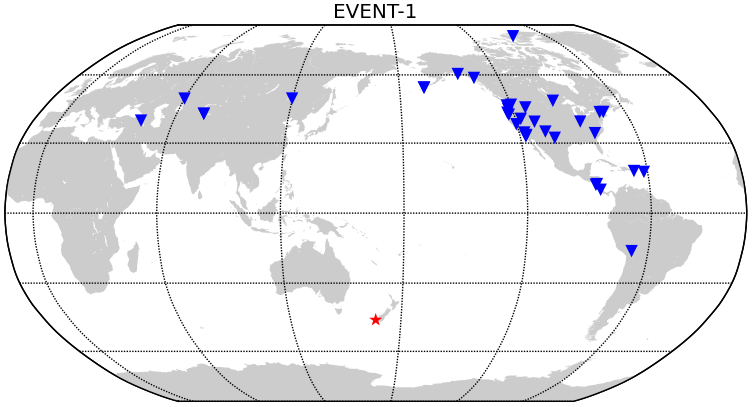
\includegraphics[width=444pt, height=240pt, keepaspectratio=true]{AXISEMTutorial-fig006.png}
% %%\caption{This should be the caption for \texttt{AXISEMTutorial-fig006.png}.}
% %%\end{figure}
% 
% {\small{}Figure A2: Event-station configuration for EVENT-1}
% \end{center}
% 
% \baselineskip=13pt
% \leftskip=0pt
% 2. To get an overview on both real data and pre-simulated seismograms: (e.g. PREM\_ANISO 
% for 5 seconds dominant period) [Figure A3]
% \begin{verbatim}
%     $ plot_seismograms.py EVENT-1/AXISEM/PREM_ANISO_5sec
% \end{verbatim}
% 
% 3.Cut the waveforms for Pdiff and PKiKP seismic phases and plot the seismograms: 
% (compared with real data)
% \begin{verbatim}
%     $ plot_seismograms.py EVENT-1/AXISEM/PREM_ANISO_5sec Pdiff
%     $ plot_seismograms.py EVENT-1/AXISEM/PREM_ANISO_5sec PKiKP
% \end{verbatim}
% 
% \begin{figure}
% %%\begin{figure}[htbp]
% 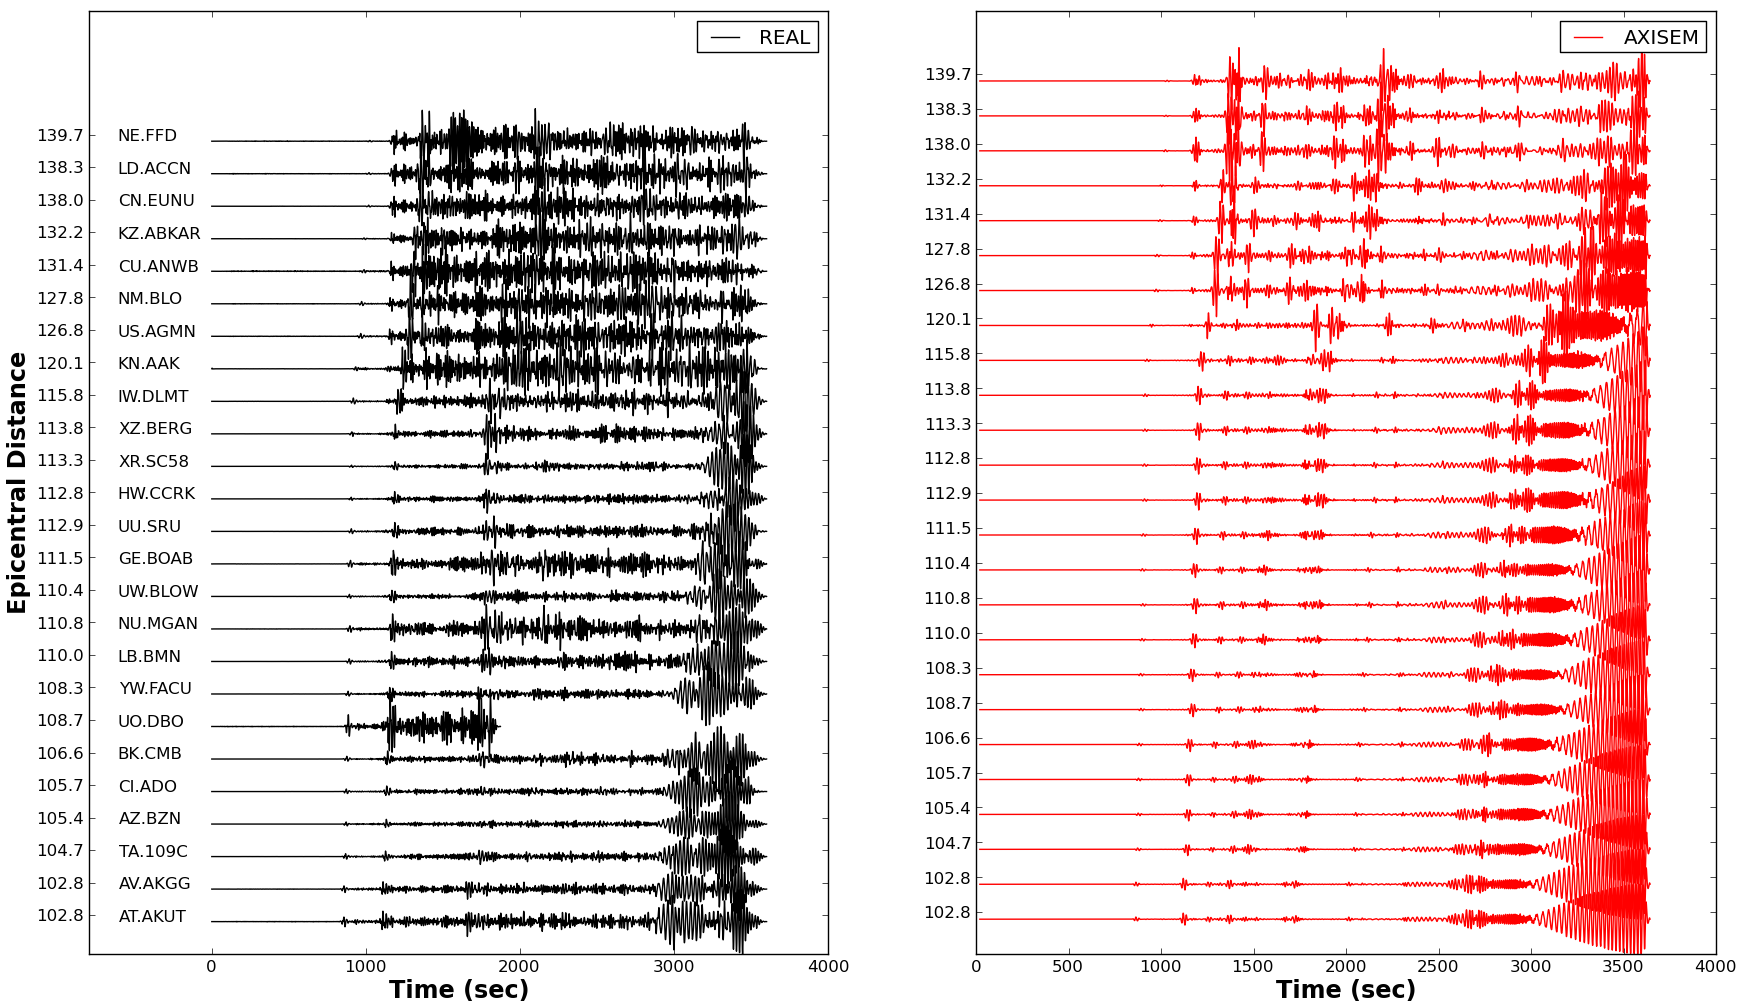
\includegraphics[width=497pt, height=287pt, keepaspectratio=true]{AXISEMTutorial-fig007.png}
% %%\caption{This should be the caption for \texttt{AXISEMTutorial-fig007.png}.}
% %%\end{figure}
% \begin{center}
% {\small{}Figure A3:Real and AXISEM waveforms for EVENT-1}
% \end{center}
% \end{figure}
% 
% \begin{figure}
% \centering
% \begin{minipage}{.5\textwidth}
%   \centering
%   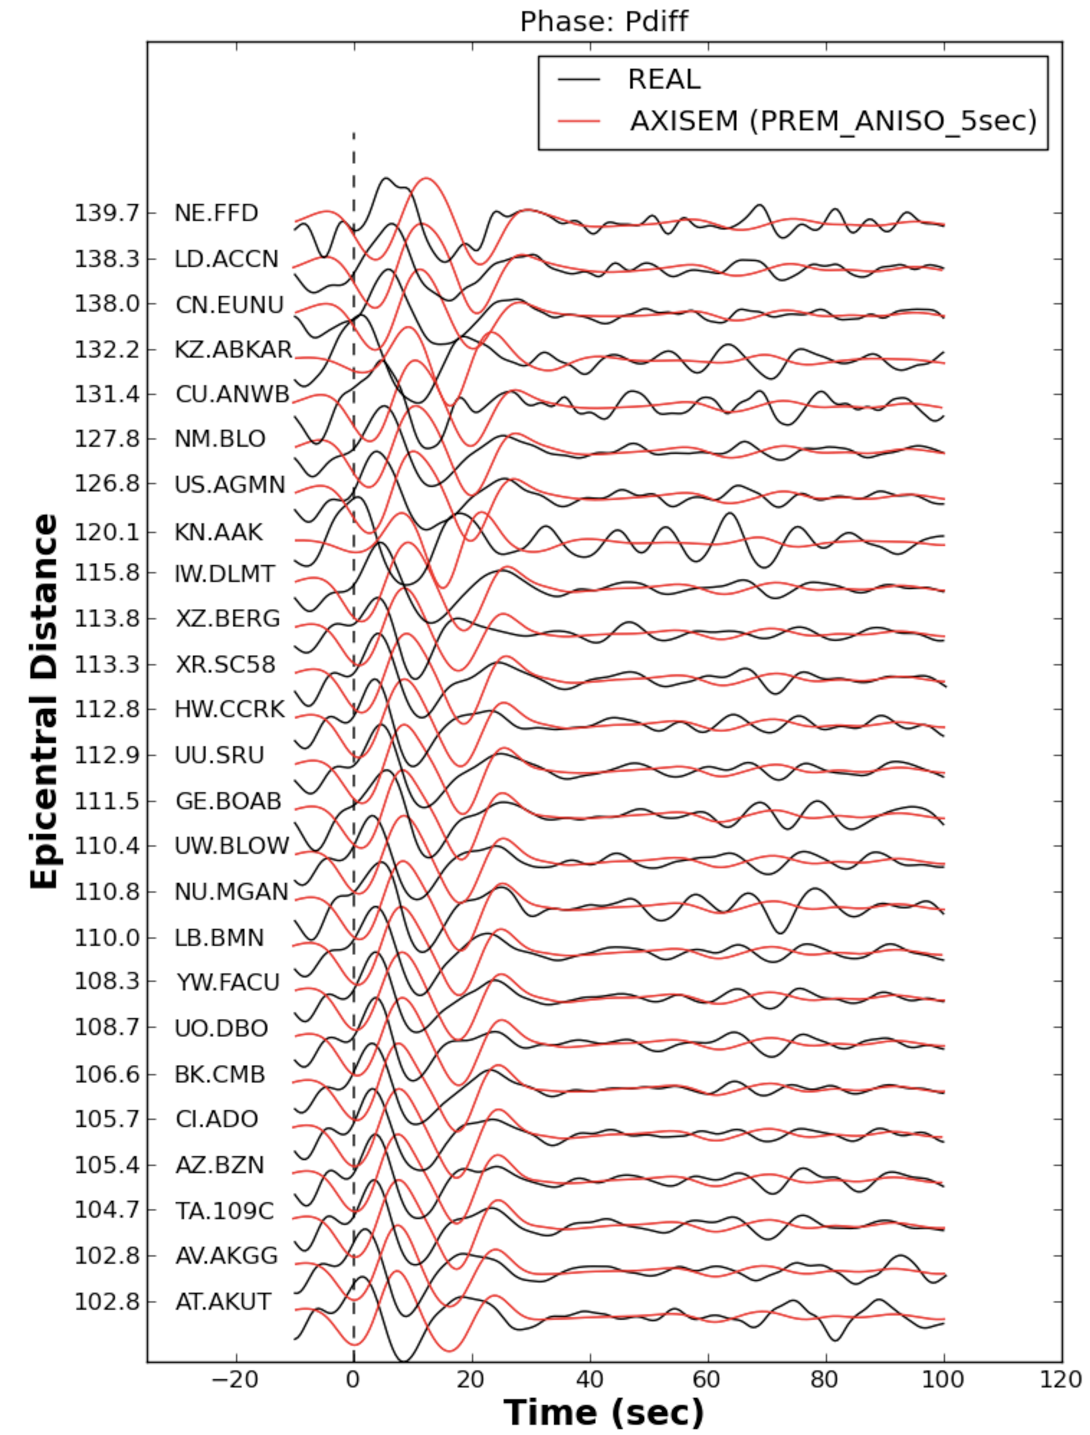
\includegraphics[width=1.\linewidth]{AXISEMTutorial-fig008.pdf}
%   %\includegraphics[width=.4\linewidth]{image1}
% \end{minipage}%
% \begin{minipage}{.5\textwidth}
%   \centering
%   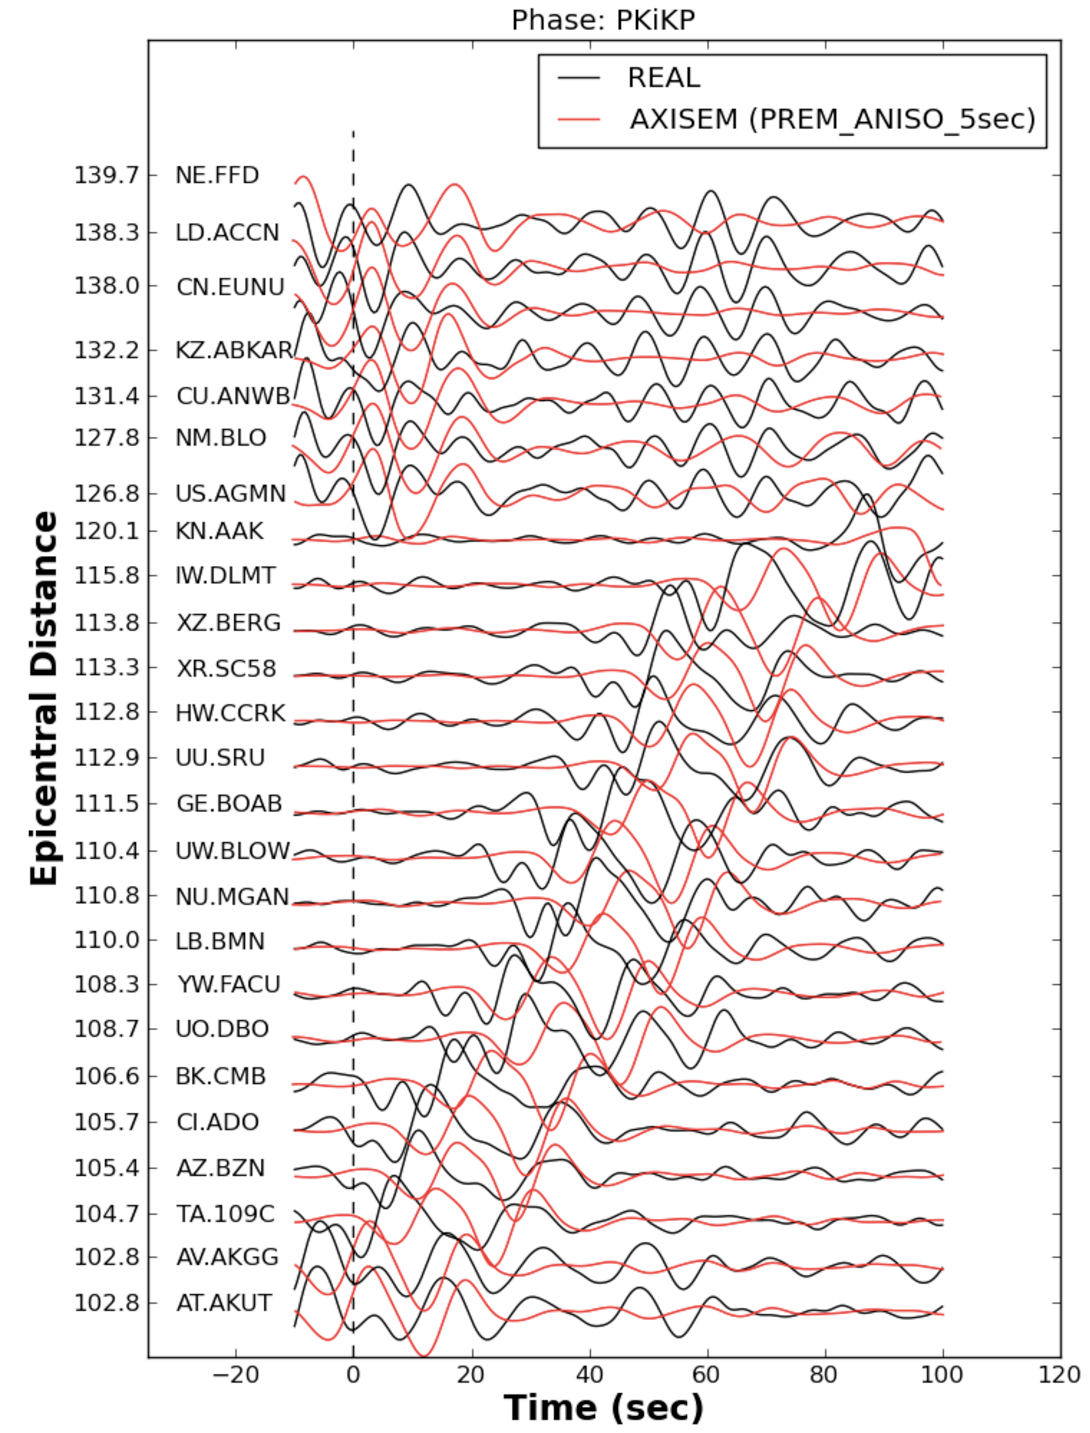
\includegraphics[width=1.\linewidth]{AXISEMTutorial-fig009.pdf}
% %   \includegraphics[width=.4\linewidth]{image1}
% \end{minipage}
% \begin{center}
% {\small{}Figure A4: Comparison between real and synthetic waveforms for Pdiff and 
% PKiKP phases. (without alignment)}
% \end{center}
% \end{figure}
% 
% 
% 4. Change the filter in \textit{plot\_seismograms.py} script and compare the results with 
% \textit{SPECFEM3D}: (for changing the filter, open \textit{plot\_seismograms.py} and change 
% values at top of the file) \\
% For this example, ????? we change hfreq (high frequency) in line 34 to 0.05Hz (20sec) and \textit{lfreq }to 0.01Hz: (Figure 
% A5)
% 
% \begin{verbatim}
%     $ plot_seismograms.py EVENT-1/AXISEM/PREM_ANISO_5sec Pdiff specfem3d
%     $ plot_seismograms.py EVENT-1/AXISEM/PREM_ANISO_5sec PKiKP specfem3d
% \end{verbatim}
% 
% 
% \begin{figure}
% \centering
% \begin{minipage}{.5\textwidth}
%   \centering
%   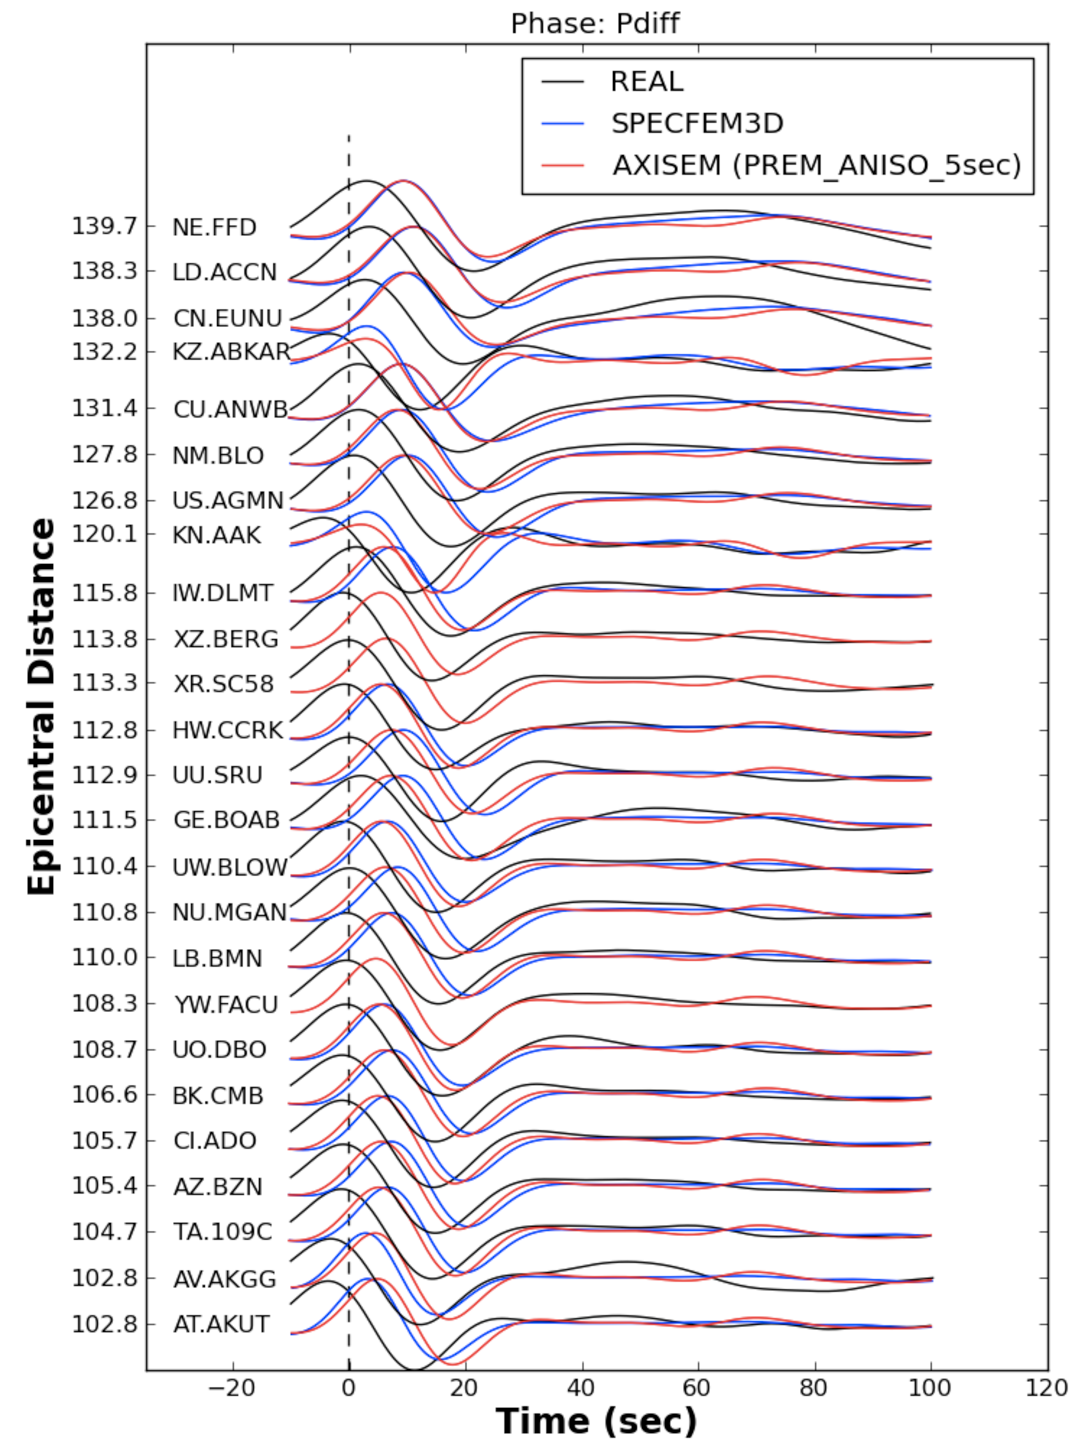
\includegraphics[width=1.\linewidth]{AXISEMTutorial-fig010.pdf}
%   %\includegraphics[width=.4\linewidth]{image1}
% \end{minipage}%
% \begin{minipage}{.5\textwidth}
%   \centering
%   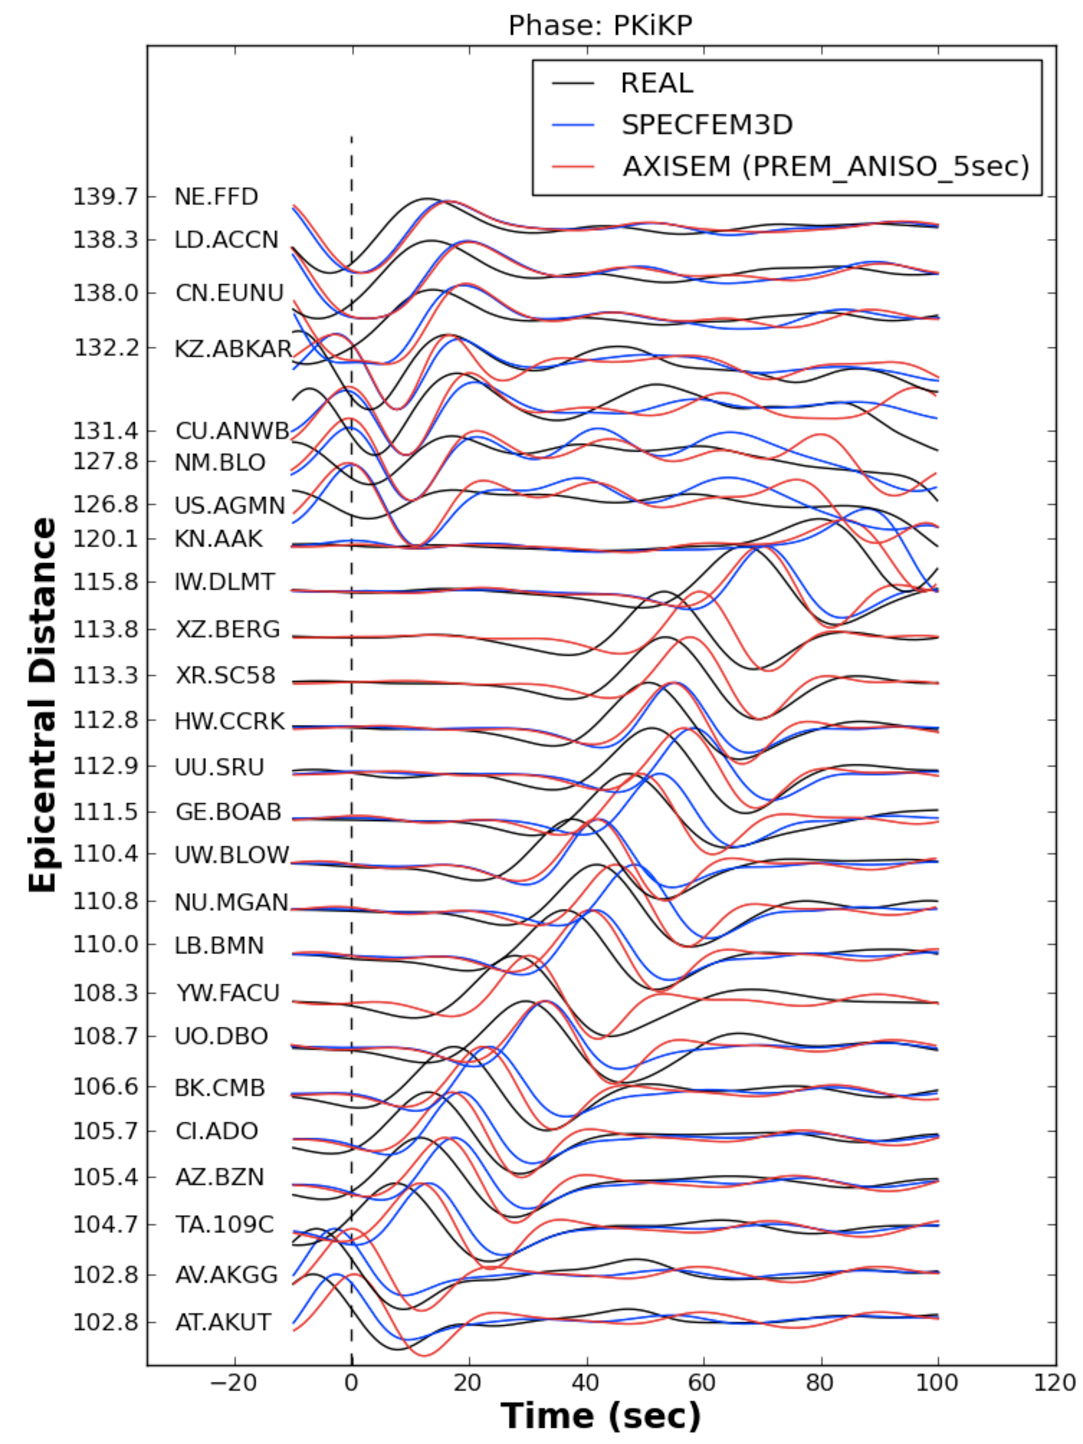
\includegraphics[width=1.\linewidth]{AXISEMTutorial-fig011.pdf}
% %   \includegraphics[width=.4\linewidth]{image1}
% \end{minipage}
% \begin{center}
% {\small{}Figure A5: Comparison between real, AXISEM and SPECFEM3D waveforms for 
% Pdiff and PKiKP phases.}
% \end{center}
% \end{figure}
% 
% 5. Compare the results of two different background models (\textit{PREM\_ANISO\_5sec} with 
% \textit{IASP91\_5sec)} for Pdiff phase: (Figure A6).
% 
% \begin{verbatim}
%     $ plot_seismograms.py EVENT-1/AXISEM/PREM_ANISO_5sec Pdiff 
%     EVENT-1/AXISEM/IASP91_5sec
% \end{verbatim}
% 
% 6. Change the filter, as explained in step 4, and repeat step 5. Here, we increase 
% the \textit{hfreq} to 0.2Hz and \textit{lfreq} to 0.05Hz (Figure A7).
% 
% \begin{figure}
% \centering
% %%\begin{figure}[htbp]
% 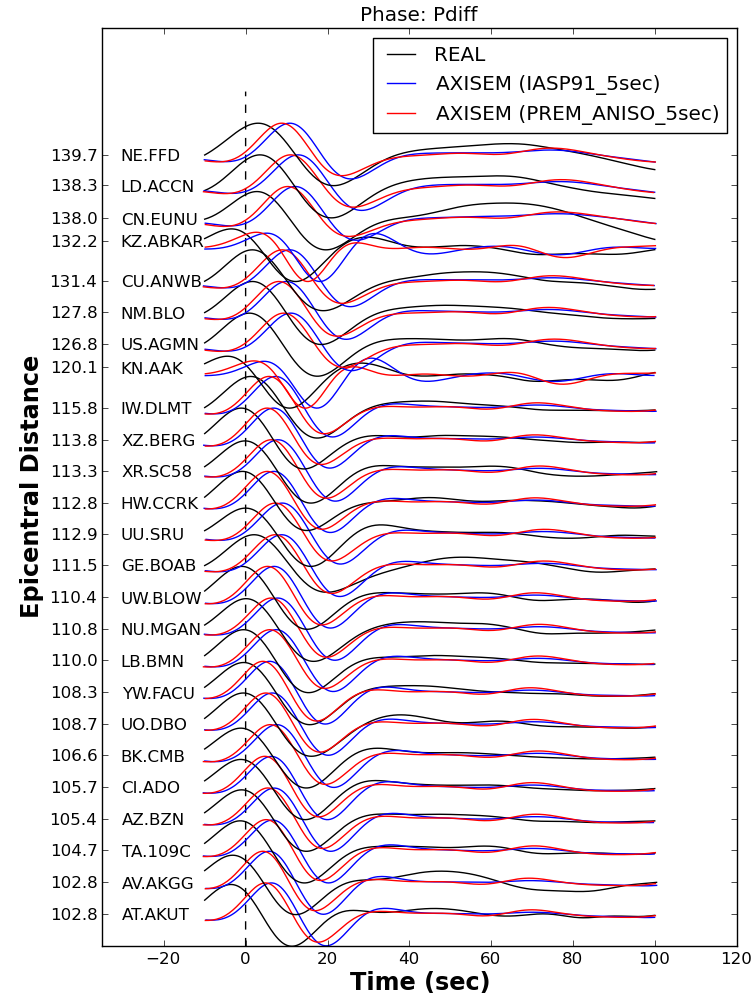
\includegraphics[width=234pt, height=310pt, keepaspectratio=true]{AXISEMTutorial-fig012.png}
% \begin{center}
% {\small{}Figure A6: Comparison between real and AXISEM waveforms for two different 
% background models (Pdiff).}
% \end{center}
% \end{figure}
% 
% \begin{figure}
% \centering
% %%\begin{figure}[htbp]
% 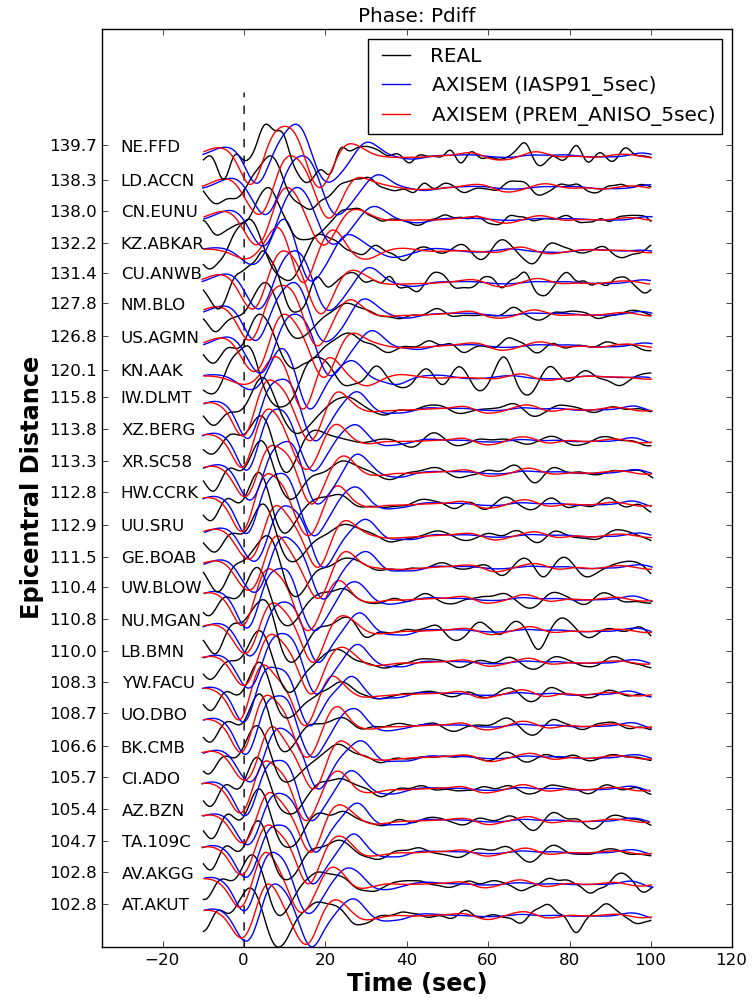
\includegraphics[width=241pt, height=320pt, keepaspectratio=true]{AXISEMTutorial-fig013.png}
% \begin{center}
% {\small{}Figure A7: Comparison between real and AXISEM waveforms for two different 
% background models (Pdiff).} 
% \end{center}
% \end{figure}
% 
% 7. Compare the seismograms calculated for two different source parameters (PREM\_ANISO\_5sec and \\
% PREM\_ANSIO\_5sec\_GCMT) for Pdiff phase: (For more information about the source 
% parameters, refer to Appendix-1) [Figure A8]
% 
% \begin{verbatim}
%     $ plot_seismograms.py EVENT-1/AXISEM/PREM_ANISO_5sec Pdiff 
%     EVENT-1/AXISEM/PREM_ANISO_5sec_GCMT
% \end{verbatim}
% 
% \begin{figure}
% \centering
% 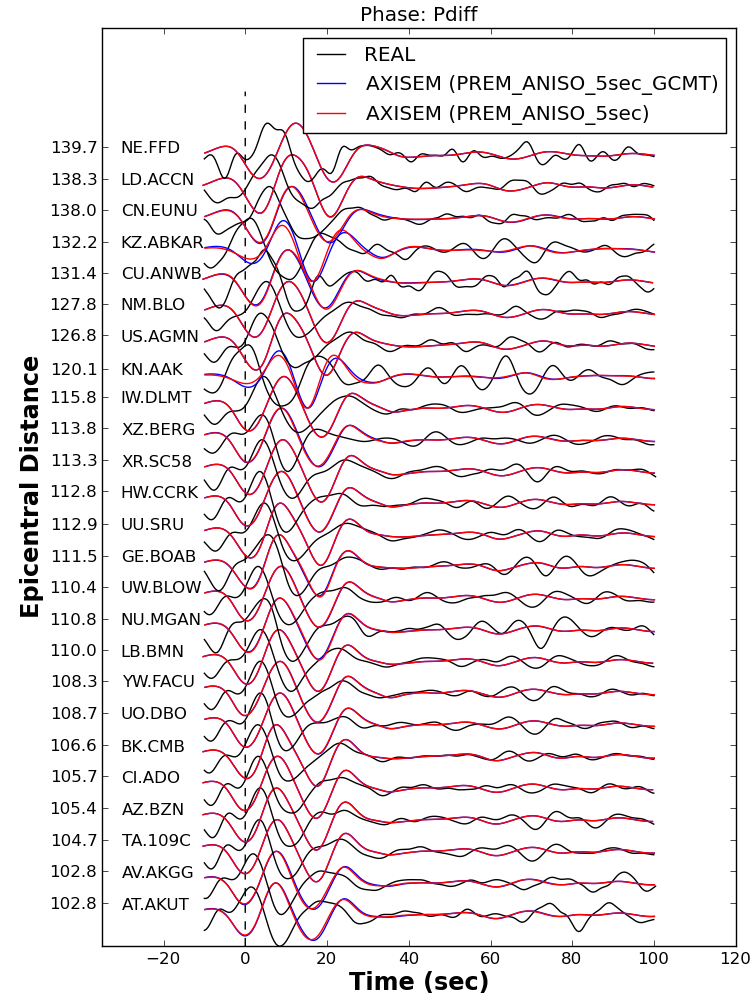
\includegraphics[width=234pt, height=310pt, keepaspectratio=true]{AXISEMTutorial-fig014.png}
% \begin{center}
% {\small{}Figure A8: Comparison between real and AXISEM waveforms for two different 
% source parameters (Pdiff).}
% \end{center}
% \end{figure}
% 
% 8. Change the filter, as explained in step 4, and repeat step 7. ????? Here, we decrease 
% the \textit{hfreq} to 0.05Hz and \textit{lfreq} to 0.01Hz. (Figure A9)
% 
% 9. Find the time shift between the synthetics and real data, shift the synthetics 
% accordingly and plot the results: (Figure A10)
% 
% \begin{verbatim}
%     $ plot_seismograms.py EVENT-1/AXISEM/PREM_ANISO_5sec Pdiff shift_synthetics
% \end{verbatim}
% 
% \vspace{13pt}
% 10. Map the calculated time shifts in step 9 on the station locations: (note that 
% it always plots the results of the latest comparison, i.e. Pdiff here) 
% 
% \begin{verbatim}
%     $ plot_travel_time_map.py EVENT-1
% \end{verbatim}
% 
% \begin{center}
% %%\begin{figure}[htbp]
% 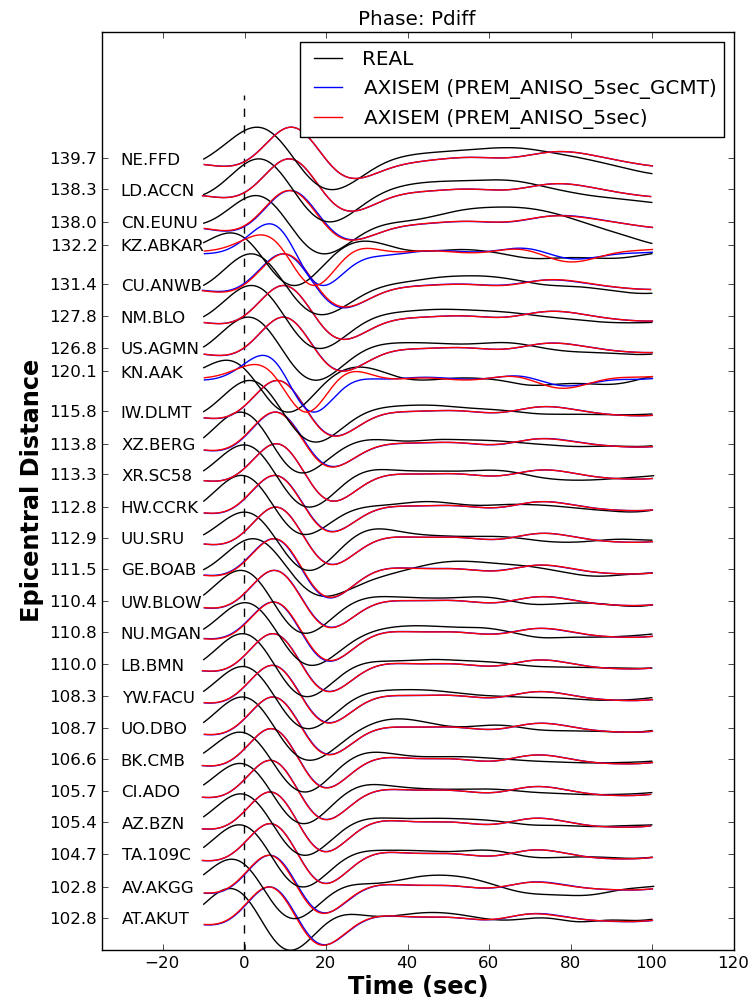
\includegraphics[width=242pt, height=322pt, keepaspectratio=true]{AXISEMTutorial-fig015.png}
% %%\caption{This should be the caption for \texttt{AXISEMTutorial-fig015.png}.}
% %%\end{figure}
% 
% {\small{}Figure A9: Comparison between real and AXISEM waveforms for two different 
% source parameters (Pdiff).}
% 
% %%\begin{figure}[htbp]
% 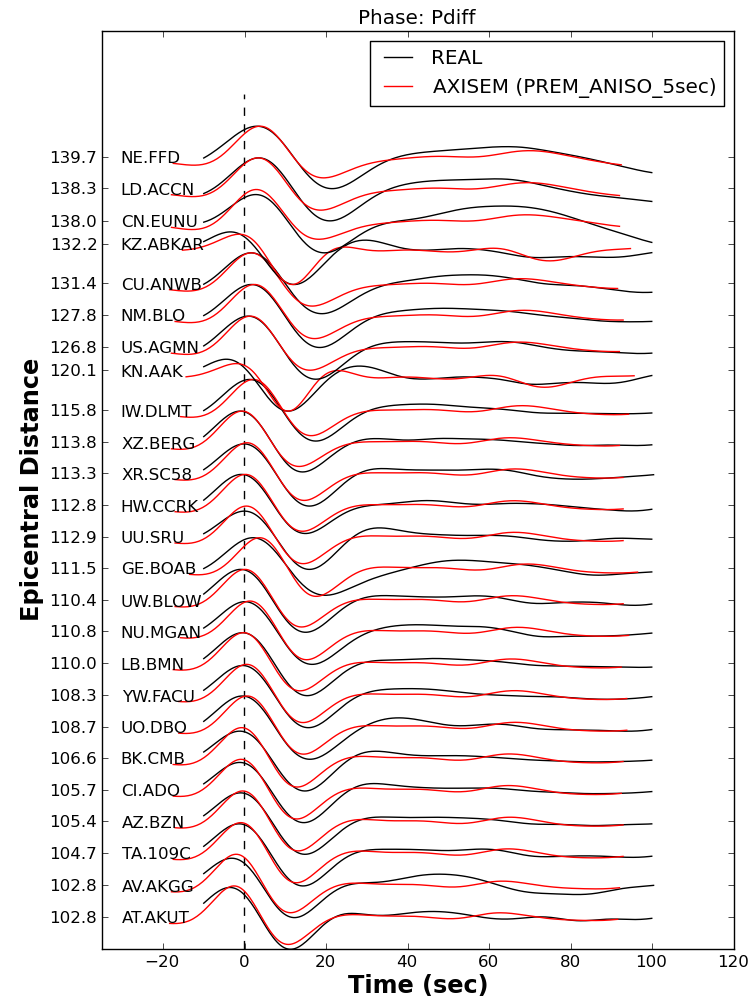
\includegraphics[width=249pt, height=331pt, keepaspectratio=true]{AXISEMTutorial-fig016.png}
% %%\caption{This should be the caption for \texttt{AXISEMTutorial-fig016.png}.}
% %%\end{figure}
% 
% {\small{}Figure A10: Comparison between real and AXISEM waveforms for Pdiff. AXISEM 
% waveforms are shifted in order to gain the maximum cross correlation coefficient.}
% 
% \vspace{1cm}
% 
% %%\begin{figure}[htbp]
% 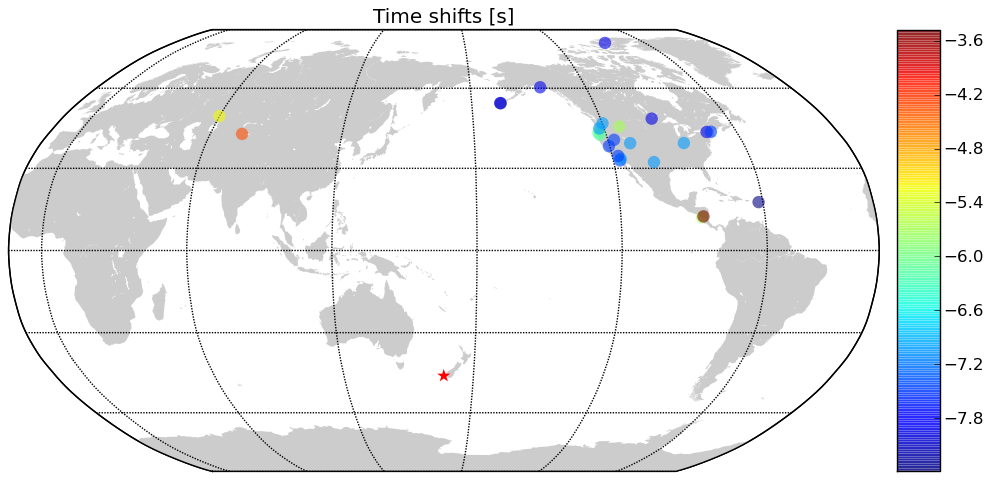
\includegraphics[width=446pt, height=217pt, keepaspectratio=true]{AXISEMTutorial-fig017.png}
% %%\caption{This should be the caption for \texttt{AXISEMTutorial-fig017.png}.}
% %%\end{figure}
% 
% {\small{}Figure A11: Time shift calculated by cross correlation between real and 
% AXISEM waveforns. Blue color indicates that Pdiff in real data arrived sooner than 
% that in the synthetic one.}
% \end{center}
% 
% \baselineskip=13pt
% \leftskip=0pt

\end{document}
